\documentclass{sig-alternate-2013}
\newfont{\mycrnotice}{ptmr8t at 7pt}
\newfont{\myconfname}{ptmri8t at 7pt}
\let\crnotice\mycrnotice%
\let\confname\myconfname%

\permission{Permission to make digital or hard copies of all or part of this work for personal or classroom use is granted without fee provided that copies are not made or distributed for profit or commercial advantage and that copies bear this notice and the full citation on the first page. Copyrights for components of this work owned by others than ACM must be honored. Abstracting with credit is permitted. To copy otherwise, or republish, to post on servers or to redistribute to lists, requires prior specific permission and/or a fee. Request permissions from permissions@acm.org.}
\conferenceinfo{WSDM'14,}{February 24--28, 2014, New York, New York, USA.}
\copyrightetc{Copyright 2014 ACM \the\acmcopyr}
\crdata{978-1-4503-2351-2/14/02\ ...\$15.00.\\
http://dx.doi.org/10.1145/2556195.2556224}

\clubpenalty=10000
\widowpenalty = 10000




\usepackage[T1]{fontenc} 
\usepackage{textcomp}

\usepackage{datetime}
\usepackage{graphicx}
\usepackage{balance}
\usepackage{float}
\usepackage{xspace}
\usepackage[numbers,sort&compress,square]{natbib}
\makeatletter
\renewcommand\bibsection%
{
  \section{\MakeUppercase{\refname}
    \@mkboth{\MakeUppercase{\refname}}{\MakeUppercase{\refname}}}
}
\makeatother

% space saving commands and packages
\usepackage{times} 
\usepackage[font=small]{caption,subfig}
%\setlength{\bibsep}{8.0pt} % natbib
\renewcommand\floatpagefraction{.9}
\renewcommand\topfraction{.9}
\renewcommand\bottomfraction{.9}
\renewcommand\textfraction{.1}   
\setcounter{totalnumber}{50}
\setcounter{topnumber}{50}
\setcounter{bottomnumber}{50}

\usepackage{booktabs}
\usepackage{amsfonts}
\usepackage{amsmath}
\usepackage{amssymb}
\usepackage{dsfont}
\usepackage{mathtools}
%%\usepackage{subfig}
\usepackage{multirow}
\usepackage{bigstrut}
\usepackage{url}
\usepackage[ruled,linesnumbered]{algorithm2e}
\usepackage{mdwlist}
\usepackage{cleveref}


\DeclareCaptionType{copyrightbox}

\newtheorem{corol}{Corollary}
\newtheorem{lemma}{Lemma}
\newtheorem{theorem}{Theorem}

\newdef{definition}{Definition}

\def\XXX{{\bf XXX}}
\def\MR{{\bf MR}}
\def\EK{{\bf EK}}

\def\betw{\mathsf{b}}
\def\kboundbetw{\mathsf{bb}}
\def\kpathbetw{\mathsf{pb}}
\def\prob{\pi}
\def\range{\mathcal{R}}
\def\TOPK{\mathsf{TOP}}
\def\VC{\mathsf{VC}}
\def\VD{\mathsf{VD}}

\newif\ifproof
\prooffalse

\begin{document}
%\conferenceinfo{WSDM} {'14, February 24--28, 2014, New York, NY, USA.}
%\CopyrightYear{2014}
%\crdata{978-1-4503-1156-4/12/10}
%\clubpenalty=10000
%\widowpenalty = 10000

\title{Fast Approximation of Betweenness Centrality \\through Sampling}
\numberofauthors{2} 
\author{
\alignauthor
Matteo Riondato\\ %\titlenote{Contact Author}\\
       \affaddr{Dept.~of Computer Science}\\
       \affaddr{Brown University}\\
       \affaddr{Providence, RI, USA}\\
       \email{matteo@cs.brown.edu}
\alignauthor
Evgenios M. Kornaropoulos\\
       \affaddr{Dept.~of Computer Science}\\
       \affaddr{Brown University}\\
       \affaddr{Providence, RI, USA}\\
       \email{evgenios@cs.brown.edu}
}
%\additionalauthors{}
\date{\today}

\maketitle
%{\bf \large \today, \currenttime}
%\vspace{-2pt}
\begin{abstract}
  %We present an efficient randomized algorithm for approximating the {\sl
  %betweenness centrality} of all nodes in a network within strict probabilistic
  %guarantees.
  Betweenness centrality is a fundamental measure in social network
  analysis, %, %quantifying
  expressing the importance or influence of individual vertices in a
  network in terms of the fraction of shortest paths that pass through them. 
  %The fastest known algorithm to
  %compute the exact betweenness of all vertices in a graph $G=(V,E)$ in
  %$O(|V|\cdot|E|)$ steps in the unweighted case and in
  %$O(|V|\cdot|E|+|V|^2\log|V|)$ steps in weighted graphs. 
  Exact computation in large networks %with millions of vertices and hundred of millions of edges 
  is prohibitively expensive and fast approximation algorithms are required in
  these cases. 
  We present two efficient randomized %approximation 
  algorithms for betweenness
  estimation. The algorithms are based on random sampling of shortest paths and
  offer probabilistic guarantees on the quality of the approximation. 
  %One algorithm computes an $(\varepsilon,\delta)$-approximation of the vector
  %of betweenness centrality of all the vertices in the graph.
  The first algorithm estimates the betweenness of all vertices: all
  approximated values are within an additive factor $\varepsilon$ from the real
  values, with probability at least $1-\delta$. The second algorithm focuses on
  the top-K vertices with highest betweenness and approximate their betweenness
  within a multiplicative factor $\varepsilon$, with probability at least
  $1-\delta$. This is the first algorithm that can compute such approximation for
  the top-K vertices. We use results from the VC-dimension theory to develop
  bounds to the sample size needed to achieve the desired approximations. By
  proving upper and lower bounds to the VC-dimension of a range set associated
  with the problem at hand, we obtain a sample size that is independent from the
  number of vertices in the network and only depends on a characteristic
  quantity that we call the vertex-diameter, that is the maximum number of
  vertices in a shortest path. In some cases, the sample size is completely
  independent from any property of the graph.
  %Extensive experimental evaluation on real and artificial networks demonstrate
  %the practicality of our methods and their performances compared to exact and
  %approximated approximated algorithms.
  The extensive experimental evaluation that we performed using real and
  artificial networks shows that our algorithms are significantly faster and
  much more scalable as the number of vertices in the network grows than
  previously presented algorithms with similar approximation guarantees.
\end{abstract}
  
%\vspace{-9pt}
\category{G.2.2}{Discrete Mathematics}{Graph Theory}[Graph algorithms]
\category{H.2.8}{Database Management}{Database Applications}[Data mining]
%\vspace{-10pt}
%\terms{Algorithms, Performance, Theory, Experimentation}
\vspace{-0.65pt}
\keywords{Betweenness centrality, graph mining, range set, sampling, social
network analysis, VC-dimension, vertex diameter}  

\section{Introduction}\label{sec:intro}
Centrality indices are fundamental metrics for network analysis. They express the
relative importance of a vertex in the network. Some of them, e.g., degree
centrality, reflect local properties of the underlying graph, while others,
like betweenness centrality, give information about the global network
structure, as they are based on shortest path computation and counting~\citep{Newman10}. In
this work we are interested in \emph{betweenness
centrality}~\citep{Anthonisse71,Freeman77}, that is, for every vertex in the
graph, the fraction of shortest paths that goes through that vertex (see
Section~\ref{sec:prelims} for formal definitions)
\ifproof
, and on some variants of it~\citep{OpsahlAS10,BorgattiE06,Brandes08}. %
\else
. %
\fi
Betweenness centrality has been used to analyze social and protein interaction
networks, to evaluate traffic in communication networks, and to identify
important intersections in road networks~\citep{Newman10,GeisbergerSS08}. There
exist polynomial-time algorithms to compute the exact betweenness
centrality~\citep{Brandes01}, but they are not practical for the analysis of the
very large networks that are of interest these days. Graphs representing online
social networks, communication networks, and the web graph have millions of
nodes and billions of edges, making a polynomial-time algorithm too expensive in
practice. Given that data mining is exploratory in nature, approximate results
are usually sufficient, especially if the approximation error is guaranteed to
be within user-specified limits. In practice, the user is interested in the
relative ranking of the vertices according to their betweenness, rather than the
actual value of the betweenness, so a very good estimation of the value of each
vertex is sufficiently informative for most purposes. It is therefore natural to
develop algorithms that trade off accuracy for speed and efficiently compute
high-quality approximations of the betweenness of the vertices.  Nevertheless,
in order for these algorithms to be practical it is extremely important that
they scale well and have a low runtime dependency on the size of the network
(number of vertices and/or edges).

\paragraph*{Our contributions} 
We present two randomized algorithms to approximate the betweenness centrality
(and some of its variants) of the vertices of a graph. The first algorithm
guarantees that the estimated betweenness values for all vertices are within an
\emph{additive} factor $\varepsilon$ from the real values, with probability at
least $1-\delta$. The second algorithm focuses on the top-$K$ vertices with
highest betweenness and returns a \emph{superset} of the top-$K$,
while ensuring that the estimated betweenness for all returned vertices is
within a \emph{multiplicative} factor $\varepsilon$ from the real value, with
probability at least $1-\delta$. This is the first algorithm to reach such a
high-quality approximation for the set of top-$K$ vertices. The algorithms are
based on random sampling of shortest paths. The analysis to derive the
sufficient sample size is novel and uses notions and results from VC-dimension
theory. We define a range set associated with the problem at hand and prove strict
bounds to its VC-dimension. The resulting sample size \emph{does not
depend on the size of the graph}, but only on the maximum number of vertices
in a shortest path, a \emph{characteristic quantity} of the graph that we call
the \emph{vertex-diameter}. For some networks, we show that the VC-dimension is
actually
at most a constant and so the sample size depends \emph{only on the approximation
parameters} and not on any property of the graph, a somewhat surprising fact
that points out interesting insights. Thanks to the lower runtime dependency on
the size of the network, our algorithms are \emph{much faster and more scalable}
than previous contributions~\citep{JacobKLPT05,BrandesP07,GeisbergerSS08}, while
offering the same approximation guarantees. Moreover, the amount of work
performed by our algorithms per sample is also less than that of others algorithms.
We extensively evaluated our methods on real graphs and compared their
performances to the exact algorithm for betweenness centrality~\citep{Brandes01}
and to other sampling-based approximation
algorithms~\citep{JacobKLPT05,BrandesP07,GeisbergerSS08}, showing that our
methods achieve a huge speedup (3 to 4 times faster) and scale much better as
the number of vertices in the network grows.

We present related work in Sect.~\ref{sec:prevwork}. Section~\ref{sec:prelims}
introduces all the basic definitions and results that we will use throughout the
paper. A range set for the problem at hand and the bounds to its VC-dimension
are presented in Sect.~\ref{sec:rangeset}. Based on these results we develop and
analyze algorithms for betweenness estimation that we present in
Sect.~\ref{sec:algo}. % 
\ifproof
Extensions of our methods to various variants of the problem are presented in
Sect.~\ref{sec:variants}. %
\fi 
Section~\ref{sec:exper} reports the methodology and
the results of our extensive experimental evaluation.

\section{Related work}\label{sec:prevwork}
Over the years, a number of centrality measures have been defined~\citep{Newman10}. In this work
we focus on betweenness centrality and some of its variants. 

Betweenness centrality was introduced in the sociology
literature~\citep{Anthonisse71,Freeman77}. \citet{Brandes08} presents a number
of minor variants. A particularly interesting one, $k$-bounded-distance
betweenness, limits the length of the shortest paths considered when computing
the centrality~\citep{BorgattiE06,Brandes08,PfefferC12}. This is not to be
confused with $k$-path betweenness centrality defined
by~\citet{KourtellisASIT12}, which considers simple random walks that are not
necessarily shortest paths. \citet{DolevEP10} present a generalization of
betweenness centrality which takes into account routing policies in the network. %
\ifproof
\citet{OpsahlAS10} define a new distance function between pair of vertices in
order to penalize paths with a high number of hops in weighted network. This
function induces a generalized and parametrized definition of betweenness.
\fi

The need of fast algorithms to compute the betweenness of vertices in a graph
arose as large online social networks started to appear. \citet{Brandes01} presents the
first efficient algorithm for the task, running in time $O(nm)$ on
unweighted graphs and $O(nm+n^2\log n)$ on weighted ones. The
algorithm computes, for each vertex $v$, the shortest path to every other vertex
and then traverses these paths backwards to efficiently compute the contribution
of the shortest paths from $v$ to the betweenness of other vertices. For very
large networks, the cost of this algorithm would still be prohibitive in
practice, so many approximation algorithms were
developed~\citep{JacobKLPT05,BrandesP07,BaderKMM07,GeisbergerSS08,MaiyaBW10,LimMRTB11}.
The use of random sampling was one of the more natural approaches to speed up
the computation of betweenness. Inspired by the work of~\citet{EppsteinW04},
\citet{JacobKLPT05} and independently \citet{BrandesP07} present an algorithm
that mimics the exact one, with the difference that,
instead of computing the contribution of all vertices to the betweenness of the
others, it only considers the contributions of some vertices sampled uniformly
at random. To guarantee that all estimates are within $\varepsilon$ from their
real value with probability at least $1-\delta$, the algorithm
from~\citep{JacobKLPT05,BrandesP07} needs $O(\log(n/\delta)/\varepsilon^2)$
samples. The analysis for the derivation of the sample size uses Hoeffding bounds~\citep{Hoeffding63} 
and the union bound~\citep{MitzenmacherU05}. 
\citet{GeisbergerSS08} noticed that this can lead
to an overestimation of the betweenness of vertices that are close to the
sampled ones and introduced different unbiased estimators that are
experimentally shown to have smaller variance and do not suffer from this
overshooting. Our algorithm is different from these because we sample, each
time, a single random shortest path. %between two randomly chosen nodes. 
This leads to a much smaller sample size and less work done for each sample,
resulting in a much faster way to compute approximations of the betweenness with
the same probabilistic guarantees. 
\ifproof
Although existing algorithms \citep{BrandesP07,JacobKLPT05,GeisbergerSS08} can be extended to return a
superset of the top-$K$ vertices with highest betweenness, they only offer an
\emph{additive} approximation guarantee, while our algorithm for the top-$K$
vertices offers a \emph{multiplicative} factor guarantee, which is much
stricter. 
\fi
We delve more in the comparisons with these algorithms in
Sect.~\ref{sec:discussion} and~\ref{sec:exper}. 

A number of works explored
the use of adaptive sampling, in contrast with the previous algorithms (and
ours) which use a fixed sample size. \citet{BaderKMM07} present an adaptive
sampling algorithm which computes good estimations for the betweenness of
high-centrality vertices, by keeping track of the partial contribution of each
sampled vertex, obtained by performing a single-source shortest paths
computation to all other vertices. \citet{MaiyaBW10} use concepts from expander
graphs to select a connected sample of vertices. They estimate the betweenness
from the sample, which includes the vertices with high centrality. They build
the connected sample by adding the vertex which maximizes the number of
connections with vertices not already in the sample. Modified versions
of this algorithm and an extensive experimental evaluation appeared
in~\citep{LimMRTB11}. The algorithm does not offer any guarantee on the quality
of the approximations. Compared to these adaptive sampling approaches, our
methods ensure that the betweenness of all (or top-$K$) vertices is well
approximated, while using a fixed, predetermined amount of samples.
\citet{SaryuceSKC13} present an algorithm that pre-processes the network in
multiple ways by removing degree-1 vertices and identical vertices, and splits it
in separate components where the computation of betweenness can be performed
independently and then aggregated. They do not present an analysis of the
complexity of the algorithm. 

In the analysis of our algorithm we use results from VC-dimension
theory~\citep{VapnikC71}, a key component of statistical learning theory. We
compute an upper bound to the VC-dimension of a range set defined on shortest
paths. \citet{KranakisKRUW97} present a number of results on the VC-dimension of
various range sets for graphs (stars, connected sets of vertices, sets of
edges), but do not deal with shortest paths. \citet{AbrahamDFGW11} use
VC-dimension to speed up shortest path computation but their range set is
different from the one we use: their ground set is the set of vertices while
ours is defined on shortest paths.

\ifproof
The present work extends substantially the preliminary
version~\citep{RiondatoK14WSDM}. The proof of all the theorems and lemmas are
presented here for the first time. Examples of betweenness centrality and of the
concept of VC-dimension have been added to Sect.~\ref{sec:prelims}. A major new
contribution is a tighter analysis of the algorithm from~\citep{BrandesP07},
presented in Sect.~\ref{sec:discussion}. We also discuss many other variants of
betweenness, including edge betweenness in Sect.~\ref{sec:variants}, where we
also present a new tighter analysis of the algorithm for $k$-path betweenness
centrality by~\citep{KourtellisASIT12}.  %An expanded
%motivation for the top-$k$ algorithm opens Sect.~\ref{sec:topk}. 
%Finally, we report many additional
%results of our experimental evaluation, including results on the top-$k$
%algorithm, in Sect.~\ref{sec:exper}.
\fi

\section{Preliminaries}\label{sec:prelims}
In this section we introduce the definitions and lemmas that we will use to
develop and analyze our results throughout the paper.

\subsection{Graphs and betweenness centrality}\label{sec:graphprelims}
Let $G=(V,E)$ be a graph, where $E\subseteq V\times V$, with $n=|V|$ vertices
and $m=|E|$ edges. The graph $G$ can be directed or undirected. We assume that
there are no self-loops from one vertex to itself and no multiple edges between
a pair of vertices. Each edge $e\in E$ has a non-negative weight
$\mathsf{w}(e)$. Given a pair of distinct vertices $(u,v)\in V\times V$,
$u\neq v$, a \emph{path $p_{uv}\subseteq V$ from $u$ to $v$} is an ordered sequence of
vertices $p_{uv}=(w_1,\dotsc,w_{|p_{uv}|})$ such that $w_1=u$, $w_{|p_{uv}|}=v$ and
for each $1\le i < |p_{uv}|$, $(w_i,w_{i+1})\in E$. The vertices $u$ and $v$ are
called the \emph{end points} of $p_{uv}$ and the vertices in
$\mathsf{Int}(p_{uv})=p_{uv}\setminus\{u,v\}$ are the \emph{internal vertices of
$p_{uv}$}. The \emph{weight}
$\mathsf{w}(p_{uv})$ of a path $p_{uv}=(u=w_1,w_2,\cdots,w_{p_{|uv|}}=v)$ from
$u$ to $v$ is the sum of the weights of the edges composing the path:
$\mathsf{w}(p_{uv})=\sum_{i=1}^{|p_{uv}|-1}\mathsf{w}((w_i,w_{i+1}))$. We denote with
$|p_{uv}|$ the number of vertices composing the path and call this the
\emph{size of the path $p_{uv}$}. Note that if the weights are not all unitary,
it is not necessarily true that $\mathsf{w}(p_{uv})=|p_{uv}|-1$. A special and
degenerate path is the \emph{empty path} $p_{\emptyset}=\emptyset$, which by
definition has weight $\mathsf{w}(p_\emptyset)=\infty$, no end points, and
$\mathsf{Int}(p_\emptyset)=\emptyset$.

Given two distinct vertices $(u,v)\in V\times V$, the \emph{shortest path distance}
$d_{uv}$ between $u$ and $v$ is the weight of a path with minimum weight 
between $u$ and $v$ among all paths between $u$ and $v$. If there is no path
between $u$ and $v$, $d_{uv}=\infty$. We call a path between $u$ and $v$ with
weight $d_{uv}$ a \emph{shortest path between $u$ and $v$}. There can be
multiple shortest paths between $u$ and $v$ and we denote the set of these paths
as $\mathcal{S}_{uv}$ and the number of these paths as
$\sigma_{uv}=|\mathcal{S}_{uv}|$. If there is no path between $u$ and $v$, then
$\mathcal{S}_{uv}=\{p_\emptyset\}$\footnote{Note that even if
$p_\emptyset=\emptyset$, the set $\{p_\emptyset\}$ is not empty. It contains
one element.}.
%By definition, $\mathcal{S}_{vv}=\emptyset$.
We denote with $\mathbb{S}_G$ the union of all the $\mathcal{S}_{uv}$'s, for all
pairs $(u,v)\in V\times V$ of distinct nodes $u\neq v$: 
\[ \mathbb{S}_G=\bigcup_{\substack{(u,v)\in V\times V \\ u\neq v}}\mathcal{S}_{uv}\enspace.\]

We now define a characteristic quantity of a graph that we will use throughout
the paper.
\begin{definition}\label{def:vertexdiam}
  Given a graph $G=(V,E)$, the \emph{vertex-diameter $\VD(G)$ of $G$} is the
  size of the shortest path in $G$ with maximum size:
  \[
  \VD(G) = \max\left\{|p| ~:~ p\in \mathbb{S}_G\right\}\enspace.\]
\end{definition}
The vertex-diameter is the maximum number of vertices among all shortest paths
in $G$. If all the edge weights are unitary, then $\VD(G)$ is equal to
$\mathsf{diam}(G)+1$, where $\mathsf{diam}(G)$ is the number of edges composing
the longest shortest path in $G$. 
%\XXX Shall we make an example with a figure?

Given a vertex $v$, let $\mathcal{T}_v\subseteq\mathbb{S}_G$ be the set of all
shortest paths that $v$ is \emph{internal} to:
\[
\mathcal{T}_v=\{p\in\mathbb{S}_G ~:~ v\in\mathsf{Int}(p)\}\enspace.
\]
In this work we are interested in the \emph{betweenness centrality} of the
vertices of a graph.

%\begin{definition}[\citep{Anthonisse71,Freeman77}]\label{def:betwenness}
\begin{definition}\label{def:betwenness}
  \citep{Anthonisse71,Freeman77} Given a graph $G=(V,E)$, the \emph{betweenness
  centrality of a vertex $v\in V$} is defined as\footnote{We use the normalized
  version of betweenness as we believe it to be more suitable for presenting
  approximation results.}
  \[
  \betw(v)=\frac{1}{n(n-1)}\sum_{p_{uw}\in\mathbb{S}_G}\frac{\mathds{1}_{\mathcal{T}_v}(p)}{\sigma_{uv}}%=\frac{1}{n(n-1)}\sum_{p_{uw}\in\mathcal{T}_v}\frac{1}{|\mathcal{S}_{uw}|}
  \enspace.
  \]
\end{definition} 

\ifproof
Figure~\ref{fig:example-betw} shows an example of betweenness values for the
vertices of a (undirected, unweighted) graph. It is intuitive, by looking at the
graph, that vertices $\mathrm{b}$ and $\mathrm{g}$ should have higher
betweenness than the others, given that they somehow act as bridges between two
sides of the network, and indeed that is the case.
\begin{figure}[ht]
  \centering
  \subfloat[Example graph]{
  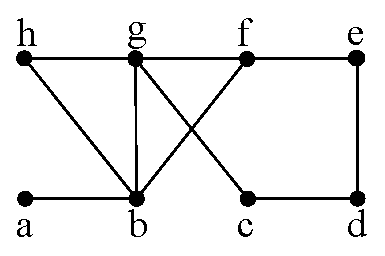
\includegraphics[width=0.2\textwidth,keepaspectratio]{figures/eps/example-betw}
  }
  \qquad
  %\hfill
 % \subfloat[Shortest paths]{
 % \begin{tabular}{ccl}
 %   \toprule
 %   From & To & Shortest Path(s) \\
 %   \midrule
 %   \multirow{6}{*}{$\mathrm{a}$} & $\mathrm{c}$ & $(\mathrm{a,b,g,c})$ \\
 %   &  $\mathrm{d}$ & $(\mathrm{a,b,g,c,d})$ \\
 %   &  $\mathrm{e}$ & $(\mathrm{a,b,f,e})$ \\
 %   &  $\mathrm{f}$ & $(\mathrm{a,b,f})$ \\
 %   &  $\mathrm{g}$ & $(\mathrm{a,b,g})$ \\
 %   &  $\mathrm{h}$ & $(\mathrm{a,b,h})$  \\
 %   \midrule
 %   \multirow{3}{*}{$\mathrm{b}$} & $\mathrm{c}$ & $(\mathrm{b,g,c})$ \\
 %   & $\mathrm{d}$ & $(\mathrm{b,g,c,d})$, $(\mathrm{b,f,e,d})$ \\
 %   & $\mathrm{e}$ & $(\mathrm{b,f,e})$ \\
 %   \midrule
 %   \multirow{3}{*}{$\mathrm{c}$} & $\mathrm{e}$ & $(\mathrm{c,d,e})$ \\
 %   & $\mathrm{f}$ & $(\mathrm{c,g,f})$ \\
 %   & $\mathrm{h}$ & $(\mathrm{c,g,h})$ \\
 %   \midrule
 %   \multirow{3}{*}{$\mathrm{d}$} & $\mathrm{f}$ & $(\mathrm{d,e,f})$ \\
 %   & $\mathrm{g}$ & $(\mathrm{d,c,g})$ \\
 %   & $\mathrm{h}$ & $(\mathrm{d,c,g,h})$ \\
 %   \midrule
 %   \multirow{2}{*}{$\mathrm{e}$} & $\mathrm{g}$ & $(\mathrm{e,f,g})$ \\
 %   & $\mathrm{h}$ & $(\mathrm{e,f,g,h})$, $(\mathrm{e,f,b,h})$ \\
 %   \midrule
 %   $\mathrm{f}$ & $\mathrm{h}$ & $(\mathrm{f,g,h})$, $(\mathrm{f,b,h})$ \\
 %   \bottomrule
 % \end{tabular}
 % }
  %\qquad
  %\subfloat[Betweenness values]{
  %\begin{tabular}{cl}
  %  \toprule
  %  Vertex & Betweenness \\
  %  \midrule
  %  a & 0 \\
  %  b & 0.250 \\
  %  c & 0.125 \\
  %  d & 0.036 \\
  %  e & 0.054 \\
  %  f & 0.080 \\
  %  g & 0.268 \\
  %  h & 0 \\
  %  \bottomrule
  %\end{tabular}
  %}
  \subfloat[Betweenness values]{
  \begin{tabular}{ccccccccc}
    \toprule
    Vertex & $\mathrm{a}$ & $\mathrm{b}$ &$\mathrm{c}$ &$\mathrm{d}$ &$\mathrm{e}$ &$\mathrm{f}$ &$\mathrm{g}$ &$\mathrm{h}$ \\
    \midrule
    $\betw(v)$ & 0 & 0.250 & 0.125 & 0.036 & 0.054 & 0.080 & 0.268 & 0 \\
    \bottomrule
  \end{tabular}
  }
  \caption{Example of betweenness values}
  \label{fig:example-betw}
\end{figure}
\fi

It is easy to see that $\betw(v)\in[0,1]$. \citet{Brandes01} presented an
algorithm to compute the betweenness centrality for all $v\in V$ in time
$O(nm)$ for unweighted graphs and $O(nm + n^2 \log n)$ for weighted graphs. 

\ifproof
We present many variants of betweenness in Sect.~\ref{sec:variants}.
\else
A ``local'' variant of betweenness, called \emph{$k$-bounded-distance
betweenness}\footnote{Bounded-distance betweenness is also known as
$k$-betweenness. We prefer the former denomination to avoid confusion with
$k$-path betweenness.} only considers
the contribution of shortest paths of size up to $k+1$~\citep{BorgattiE06,Brandes08}.
For $k>1$ and any pair of distinct vertices $u,v\in V$, $u\neq V$, let
$\mathcal{S}^{(k)}_{uv}\subseteq\mathcal{S}_{uv}$ be the set of shortest paths
from $u$ to $v$ of size at most $k+1$, with
$\sigma^{(k)}_{uv}=|\mathcal{S}^{(k)}_{uv}|$, and let $\mathbb{S}^{(k)}_G$ be the
union of all the $\mathcal{S}^{(k)}_{uv}$. Let
$\mathcal{T}^{(k)}_v\subseteq\mathcal{T}_v$ be the set of all shortest paths
\emph{of size up to $k$} that $v$ is internal to, for each $v\in V$.

%\begin{definition}[\citep{BorgattiE06,Brandes08}]\label{def:kboundbetweenness}
\begin{definition}\label{def:kboundbetweenness}
  \citep{BorgattiE06,Brandes08} Given a graph $G=(V,E)$ and an integer $k>1$,
  the \emph{$k$-bounded-distance betweenness centrality of a vertex $v\in V$} is
  defined as
  \[
  %\betw(v)=\sum_{(u,w)\in V\times
  %V}\sum_{p\in\mathcal{S}_{uw}}\frac{\mathds{1}_{\mathcal{T}_v}(p)}{|\mathcal{S}_{uw}|}\enspace.
  %\betw(v)=\sum_{p_{uw}\in\mathbb{S}_G}\frac{\mathds{1}_{\mathcal{T}_v}(p)}{|\mathcal{S}_{uw}|}\enspace.
  \kboundbetw^{(k)}(v)=\frac{1}{n(n-1)}\sum_{p_{uw}\in\mathbb{S}^{(k)}_G}\frac{\mathds{1}_{\mathcal{T}^{(k)}_v}(p)}{\sigma^{(k)}_{uw}}
  %=\frac{1}{n(n-1)}\sum_{p_{uw}\in\mathcal{T}^{(k)}_v}\frac{1}{\left|\mathcal{S}^{(k)}_{uw}\right|}
  \enspace.
  \]
\end{definition}
Other variants of centrality are presented in the extended
version~\citep{RiondatoK13}.
\fi

\subsection{Vapnik-Chervonenkis dimension}\label{sec:prelvcdim}
The Vapnik-Chernovenkis (VC) dimension of a class of subsets defined
on a set of points is a measure of the complexity or expressiveness of such
class~\citep{VapnikC71}. Given a probability distribution on the set of points,
a finite bound on the VC-dimension of the class of subsets implies a bound on
the number of random samples required to approximate the probability of each
subset in the class with its empirical average. We outline here some basic
definitions and results and refer the reader to the book by~\citet{MohriRT12}
for an in-depth presentation.
%works of~\citet[Sect.~14.4]{AlonS08} and
%\citet[Sect.~3]{BoucheronBL05} for an introduction of VC-dimension and a survey
%of recent developments. \XXX Cite book Foundations of ML instead.
%~\citet[Sect.~12.4]{DevroyeGL96},
%\citet[Sect.~3]{BoucheronBL05}, \citet[Sect.~14.4]{AlonS08}, and
%\citet{Vapnik99} for more details on VC-dimension.

Let $D$ be a domain and $\range$ be a collection of subsets from $D$. We call
$\range$ a \emph{range set on $D$}.
Given $B\subseteq D$, the \emph{projection of $\range$ on $B$} is the set 
$P_\range(B)=\{ B\cap A ~:~ A\in\range\}$. We say that the set $B$ is
\emph{shattered} by $\range$ if $P_\range(B)=2^B$.

\begin{definition}\label{def:vcdim}
  The \emph{Vapnik-Chervonenkis (VC) dimension of $\range$}, denoted as
  $\VC(\range)$, is the cardinality of the largest subset of $D$ that is
  shattered by $\range$.
\end{definition}

\ifproof
Note that a range space $(X,R)$ with an arbitrary large set of points $X$ and
an arbitrary large family of ranges $R$ can have a bounded VC-dimension. A simple
example is the family of intervals in $[0,1]$ (i.e. $X$ is all the points in
$[0,1]$ and $R$ all the intervals $[a,b]$, such that $0\leq a\leq b\leq 1$). Let
$A=\{x,y,z\}$ be the set of three points $0<x<y<z<1$. No interval in $R$ can
define the subset $\{x,z\}$ so the VC-dimension of this range space is less than
3~\citep[Lemma 10.3.1]{Matousek02}. Another example is shown in
Fig.~\ref{fig:rectangles}.
\begin{figure}[ht]
  \centering
  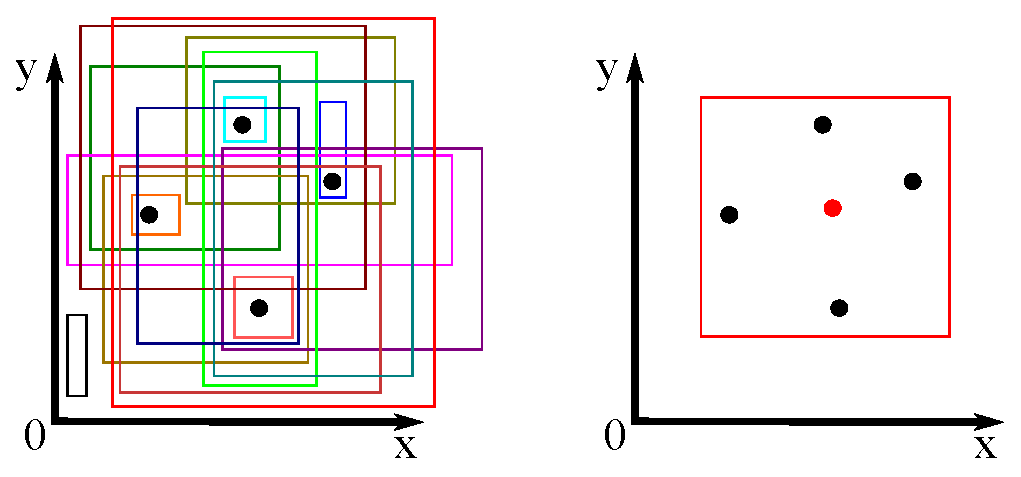
\includegraphics[width=.7\textwidth,keepaspectratio]{figures/rectangles}
  \caption{Example of range space and VC-dimension. The space of points is the
  plane $\mathbb{R}^2$ and the set $R$ of ranges is the set of all
  \emph{axis-aligned rectangles}. The figure on the left shows graphically that
  it is possible to shatter a set of four points using 16 rectangles. On the
  right instead, one can see that it is impossible to shatter five points, as,
  for any choice of the five points, there will always be one (the red point in
  the figure) that is internal to the convex hull of the other four, so it would
  be impossible to find an axis-aligned rectangle containing the four points
  but not the internal one. Hence $\VC((\mathbb{R}^2,R))=4$.}
  \label{fig:rectangles}
\end{figure}
\fi

The main application of VC-dimension in statistics and learning
theory is in computing the number of samples needed to approximate the
probabilities of the ranges using their empirical averages as
unbiased estimators. Formally, let $X_1^k=(X_1,\dotsc,X_k)$ be a collection of
independent identically distributed random variables taking values in $D$,
sampled according to some distribution $\phi$ defined on the elements of $D$.
For a set $A\subseteq D$, let $\phi(A)$ be the probability that a sample from
$\phi$ belongs to the set $A$, and let the \emph{empirical average} of $\phi(A)$
on $X_1^k$ be 
\[
\phi_{X_1^k}(A)=\frac{1}{k}\sum_{j=1}^k\mathds{1}_A(X_j)\enspace.%, 
\]
%where $\mathds{1}_A$ is the indicator function for the set $A$. 
The empirical average of $\phi(A)$ can be used as an \emph{unbiased} estimator
for $\phi(A)$.

\begin{definition}\label{def:eapprox}
  Let $\range$ be a range set on %a domain
  $D$ and $\phi$ be a probability distribution on $D$. For $\varepsilon\in(0,1)$,
  an \emph{$\varepsilon$-approximation to $(\range,\phi)$} is a bag $S$ of
  elements of $D$ such that 
  \[
  \sup_{A\in\range}|\phi(A)-\phi_S(A)|\le\varepsilon\enspace.\]
\end{definition}

When an upper bound to the VC-dimension of $\range$ is available, it is possible
to build an $\varepsilon$-approximation by sampling points of
the domain according to the distribution $\phi$.

\begin{theorem}[Thm.~2.12~\citep{HarPS11} (see also~\citep{LiLS01})]\label{thm:eapprox}
  Let $\range$ be a range set on a domain $D$ with
  $\VC(\range)\le d$, and let $\phi$ be a distribution on $D$. Given
  $\varepsilon,\delta\in(0,1)$ let $S$ be a collection of $|S|$ points from $D$
  sampled according to $\phi$, with
  \begin{equation}\label{eq:vceapprox}
	|S|=\frac{c}{\varepsilon^2}\left(d+\ln\frac{1}{\delta}\right)
  \end{equation}
  where $c$ is an universal positive constant. Then $S$ is an
  $\varepsilon$-approximation to $(\range,\phi)$ with probability at least
  $1-\delta$.
\end{theorem}
%\XXX This is always a weird sentence that reviewers don't get. We should phrase it differently.
The constant $c$ is approximately $0.5$~\citep{LofflerP09}.
%\citet{LofflerP09} showed experimentally that the constant $c$ is approximately
%$0.5$. We used this value in our experiments.
%A similar definition offers relative guarantees on the approximation.
It is possible to obtain \emph{relative} guarantees on the approximation.
\begin{definition}\label{def:releapprox}
  Let $\range$ be a range set on $D$ and $\phi$ be a probability distribution on
  $D$. For $p,\varepsilon\in (0,1)$, a \emph{relative
  $(p,\varepsilon)$-approximation to $(\range,\phi)$} is a bag $S$ of elements
  from $D$ such that 
  \begin{itemize}
    \item For any $A\in\range$ such that $\phi(A)\ge p$, we have 
      \[ |\phi(A) - \phi_S(A)|\le \varepsilon\phi(A)\enspace.\]
    \item For any $B\in\range$ such that $\phi(B)< p$, we have $\phi_S(B)\le
      (1+\varepsilon)p$.
  \end{itemize}
\end{definition}

\begin{theorem}[Thm.~2.11~\citep{HarPS11}]\label{thm:releapprox}
  Let $\range$ be a range set on a domain $D$ with
  $\VC(\range)\le d$, and let $\phi$ be a distribution on $D$. Given
  $\varepsilon,\delta,p\in(0,1)$ let $S$ be a collection of $|S|$ points from $D$
  sampled according to $\phi$, with 
  \begin{equation}\label{eq:releapprox}
    |S|\ge\frac{c'}{\varepsilon^2p}\left(d\log\frac{1}{p}+\log\frac{1}{\delta}\right)
  \end{equation}
  where $c'$ is an absolute positive constant. Then $S$ is a relative
  $(p,\varepsilon)$-approximation to $(\range,\phi)$ with probability at least
  $1-\delta$.
\end{theorem}

It is important to mention that if $\VC(\range)$ and/or the upper bound $d$ do
not depend on $|D|$ or on $|\range|$ neither do the sample sizes presented in
Thm.~\ref{thm:eapprox} and~\ref{thm:releapprox}. This will make our algorithms
scale well as the size of the network increases.

\section{A range set of shortest paths}\label{sec:rangeset}
We now define a range set of the shortest paths of a graph $G=(V,E)$, and present 
a strict upper bound to its VC-dimension. %We show that this upper bound is strict. 
We use the range set and the bound in the analysis of our algorithms for estimating
the betweenness centrality of vertices of $G$.

The range set $\range_G$ is defined on the set $\mathbb{S}_G$ of all shortest
paths between vertices of $G$. It contains, for each vertex $v\in V$, the set
$\mathcal{T}_v$ of shortest paths that $v$ is internal to:
\[
\range_G = \{\mathcal{T}_v ~:~ v\in V\}\enspace.
\]

\begin{lemma}\label{lem:vcdimuppbound}
  %Given a graph $G=(V,E)$ with vertex-diameter $\Delta_G$, the range set
  %$\range_G$ associated to the shortest paths in $G$ has VC-dimension
  $\VC(\range_G)\le\lfloor\log_2(\VD(G)-2)\rfloor+1$.
\end{lemma}

\begin{proof}
%\begin{IEEEproof}
Let $\ell>\lfloor\log_2(\VD(G)-2)\rfloor+1$ and assume for the sake of contradiction
that $\VC(\range_G)=\ell$. From the definition of the VC-dimension there is a set
$Q\subseteq\mathbb{S}_G$ of size $\ell$ that is shattered by $\range_G$. Let $p$ be
an element of $Q$. There are  $2^{\ell-1}$ non-empty subsets of
$Q$ containing the path $p$. Let us label these non-empty subsets of $Q$ containing $p$ as
$S_1,\dotsc,S_{2^{\ell-1}}$, where the labelling is arbitrary.
Given that $Q$ is shattered, for each set $S_i$ there must be a range $R_i$ in
$\range_G$ such that $S_i=Q\cap R_i$. Since all the $S_i$'s are
different from each other, then all the $R_i$'s must be different from each
other. Given that $p$ belongs to each $S_i$, then $p$ must also belong to each
$R_i$, that is, there are $2^{\ell-1}$ distinct ranges in $\range_G$ containing
$p$. But $p$ belongs only to the ranges corresponding to internal vertices of
$p$, i.e., to vertices in $\mathsf{Int}(p)$. This means that the number of ranges
in $\range_G$ that $p$ belongs to is equal to $|p|-2$. But $|p|\le\VD(G)$, by
definition of $\VD(G)$, so $p$
can belong to at most $\VD(G)-2$ ranges from $\range_G$. Given that
$2^{\ell-1}>\VD(G)-2$, we reached a contradiction and there cannot be $2^{\ell-1}$
distinct ranges containing $p$, hence not all the sets $S_i$ can be expressed as
$Q\cap R_i$ for some $R_i\in\range_G$. Then $Q$ cannot be shattered and
$\VC(\range_G)\le\lfloor\log_2(\VD(G)-2)\rfloor+1$.%\qed
\end{proof}
%\end{IEEEproof}

\paragraph{Unique shortest paths}\label{sec:rangeunique}
In the restricted case when the graph is undirected and
every pair of distinct vertices has either none or a unique shortest path
between them, the VC-dimension of $\range_G$ reduces %collapses 
to a \emph{constant}. This is a
somewhat surprising result with interesting consequences. From a theoretical
point of view, it suggests that there should be other characteristic
quantities of the graph different from the vertex diameter that control the
VC-dimension of the range set of shortest paths, and these quantities are
constant on graph with unique shortest paths between vertices. From a more
practical point of view, we will see in Sect.~\ref{sec:algo} that this result has an
impact on the sample size needed to approximate %for approximating 
the betweenness centrality of
networks where the unique-shortest-path property is satisfied or even enforced,
like road networks~\citep{GeisbergerSS08}. In particular, the resulting sample
size will be \emph{completely independent} from any characteristic of the
network, and will only be a function of the parameters controlling the desired
approximation guarantees. We are currently investigating whether this result can
be extended to the case of directed graphs.
\ifproof
\else
Due to space constraints, we defer the proof to the extended online version of
the paper~\citep{RiondatoK13}.
\fi

\begin{lemma}\label{lem:vcdimuppboundunique}
  Let $G=(V,E)$ be an undirected graph with $|\mathcal{S}_{uv}|\le1$ for all
  pairs $(u,v)\in V\times V$. Then $\VC(\range_G)\le 3$.
%  Given an undirected
%  graph $G=(V,E)$ such that $|\mathcal{S}_{uv}|\le1$ for all
%  pairs $(u,v)\in V\times V$, the range set $\range_G$ of the
%  shortest paths in $G$ has VC-Dimension $\VC(\range_G)\le3$.
\end{lemma}

\ifproof
\begin{proof}
%\begin{IEEEproof}
  First of all, notice that in this restricted setting, if two different
  shortest paths $p_1$ and $p_2$ meet at a vertex $u$, then they either go on
  together or %at a certain point 
  they separate never to meet again at any other
  vertex $v\neq u$. This is easy to see: if they could separate at $u$ and then
  meet again at some $v$, then there would be two distinct shortest paths
  between $u$ and $v$, which is a contradiction of the hypothesis. Let us denote
  this fact as $\mathsf{F}$.

  Assume now that $\VC(\range_G)>3$, then there must be a set
  $Q=\{p_1,p_2,p_3,p_4\}$ of four shortest paths that can be shattered by
  $\range_G$. Then there is a vertex $w$ such that $\mathcal{T}_w\cap Q=Q$, i.e.,
  all paths in $Q$ go through $w$. Let $x$ be the farthest predecessor of $w$
  along $p_1$ that $p_1$ shares with some other path from $Q$, and let $y$ be
  the farthest successor of $w$ along $p_1$ that $p_1$ shares with some other
  path from $Q$. It is easy to see that if either $x$ or $y$ (or both) do not
  exist, then $Q$ cannot be shattered, as we would incur in a contradiction of
  fact $\mathsf{F}$. 
  
  Let us then assume that both $x$ and $y$ exist.
  Let $Q_x=\mathcal{T}_x\cap Q$ and $Q_y=\mathcal{T}_y\cap Q$.
  Because of fact $\mathsf{F}$, all paths in $Q_x$ must go through the same vertices
  between $x$ and $w$ and all paths in $Q_y$ must go through the same vertices
  between $w$ and $y$. This also means that all paths in $Q_x\cap Q_y$ must go
  through the same vertices between $x$ and $y$. If $Q_x\cup Q_y\neq Q$, let
  $p^*\in Q\setminus(Q_x\cup Q_y)$. Then from the definition of $x$ and $y$ and
  from fact $\mathsf{F}$ we have that there is no vertex $v$ such that
  $\mathcal{T}_v\cap Q=\{p_1,p^*\}$, which implies that $Q$ can not be
  shattered. 
  
  Suppose from now on that $Q_x\cup Q_y=Q$.  If $Q_x\cap Q_y=Q$, then
  all the paths in $Q$ go through the same vertices between $x$ and $y$. From
  this and the definition of $x$ and $y$ we have that there is no vertex $v$
  such that, for example, $\mathcal{T}_v\cap Q=\{p_1,p_2\}$, hence $Q$ cannot be
  shattered. Suppose instead that $Q_x\cap Q_y\neq Q$ and let $S=(Q_x\cap
  Q_y)\setminus\{p_1\}$. If $S\neq\emptyset$ then there is at least a path
  $p'\in S$ which, from the definition of $S$ and fact $\mathsf{F}$, must go
  through all the same vertices as $p_1$ between $x$ and $y$. Moreover, given
  that $Q_x\cap Q_y\neq Q$, there must be a path $p^*\in Q\setminus\{p_1\}$
  different from $p_1$ such that $p^*\notin S$. Then, from the definition of
  $x$, $y$, and $S$, and from the existence of $p'$, there can be no vertex $v$
  such that $\mathcal{T}_v\cap Q=\{p_1,p^*\}$, hence $Q$ cannot be shattered.
  Assume now that $S=\emptyset$ and consider the case $Q_x=\{p_1,p_2,p_3\}$,
  $Q_y=\{p_1,p_4\}$ (all other cases follow by symmetry with this case).
  Consider the set $\{p_1,p_3\}$. From the definition of $x$ and $Q_x$, and from
  fact $\mathsf{F}$ we have that there can not be a vertex $v$ between the end
  point of $p_1$ before $x$ and $w$ such that $\mathcal{T}_v\cap Q=\{p_1,p_3\}$.
  At the same time, from the definition of $y$ and from fact $\mathsf{F}$, we
  have that such a $v$ can not be between $w$ and the end point of $p_1$ after
  $y$. This implies that $Q$ can not be shattered.

  We showed that in all possible cases we reached a contradiction and $Q$,
  which has size $4$, can not be shattered by $\range_G$. Hence $\VC(\range_G)\le
  3$.
%\end{IEEEproof}
\end{proof}
\fi

\ifproof
\else
%\subsection{Variants}\label{sec:rangevariants}
\paragraph{Bounded-distance betweenness}
For the case of $k$-bounded-distance betweenness, if we let
$\range_G^{(k)}=\{\mathcal{T}_v^{(k)}~:~ v\in V\}$, it is easy to bound
$\VC(\range_G^{(k)})$ following the same reasoning as in
Lemma~\ref{lem:vcdimuppbound}.
\begin{lemma}\label{lem:vcdimuppboundk}
$\VC(\range_G^{(k)})\le\lfloor\log_2(k-1)\rfloor+1$.
\end{lemma}
\fi

\subsection{Tightness}\label{sec:tightness}
The bound presented in Lemma~\ref{lem:vcdimuppbound} is strict in the sense that
for each $d\ge 1$ we can build a graph $G_d$ with vertex-diameter
$\VD(G_d)=2^d+1$ and such that the range set $\range_{G_d}$ associated to the set of
shortest paths of $G_d$ has VC-dimension exactly
$d=\lfloor\log_2(\VD(G_d)-2)\rfloor+1$. 
%For the sake of clarity, we will discuss
%only the case of undirected graphs with equal edge weights, but all we say can
%be easily adapted to the general case.

\ifproof
We now introduce a class $\mathcal{G}=(G_d)_{d\ge 1}$ of graphs indexed by $d$.
The graphs in $\mathcal{G}$ are the ones for which we can show the tightness of
the bound to the VC-dimension of the associated range set.
We call the graph $G_d\in\mathcal{G}$ the \emph{$d$\textsuperscript{th} concertina graph}.
Figure~\ref{fig:tightgraphs} shows $G_1$, $G_2$, $G_3$, and $G_4$. The
generalization to higher values of $d$ is be straightforward.
By construction, $\VD(G_d)=2^d+1$, so that
$\lfloor\log_2(\VD(G_d)-2)\rfloor+1=d$. The $3(2^{d-1})$ vertices of $G_d$ can
be partitioned into three classes, \emph{top}, \emph{bottom}, and \emph{middle},
according to their location in a drawing of the graph similar to those in
Fig.~\ref{fig:tightgraphs}. $G_d$ has $2^{d-1}-1$ top vertices, $2^{d-1}-1$ bottom vertices, and
$2^{d-1}+2$ middle vertices. For each top vertex $v$, let $\mathsf{f}(v)$ be the
\emph{corresponding bottom vertex}, i.e., the bottom vertex $u$ whose neighbors
are the same middle vertices that are neighbors of $v$. Among the middle
vertices, the two with degree 1 are special and are called the \emph{end
vertices} of $G_d$ and denoted as $v_\ell$ and $v_\mathrm{r}$, where the
labels can be arbitrarily assigned. We now build a set $Q$ of $d$
shortest paths from $v_\ell$ to $v_\mathrm{r}$ and show that it is
shattered by $\range_{G_d}$, therefore proving that $\VC(\range_{G_d})\ge d$.
This fact, together with Lemma~\ref{lem:vcdimuppbound}, allows us to conclude
that $\VC(\range_{G_d})=d$. 
\else
There is a class $\mathcal{G}=(G_d)_{d\ge 1}$ of graphs indexed by d, such that
the graphs in $\mathcal{G}$ are the ones for which we can show the tightness of
the bound to the VC-dimension of the associated range set. We call the graph
$G_d\in\mathcal{G}$ the \emph{$d$-th concertina graph}.
Figure~\ref{fig:tightgraphs} shows $G_1$, $G_2$, $G_3$, and $G_4$. The
generalization to higher values of $d$ should be straightforward. Each graph
$G_d$ has $3(2^{d-1}$ vertices and vertex-diameter $d$.
\fi
\begin{lemma}\label{lem:vcdimlowbound}
  $\VC(\range_{G_d})=d$.
\end{lemma}
\ifproof
\begin{proof}
%\begin{IEEEproof}
  As we said, the $d$ paths in $Q$  go from $v_\ell$ to $v_\mathrm{r}$.
  From this and the definition of $G_d$ it should be clear that they must go through
  all the middle vertices of $G_d$. Consider now the set
  $S=2^Q\setminus\{Q,\emptyset\}$. We now build a map $\mathsf{r}$
  from the elements of $S$ to the set of top and bottom vertices of $G_d$. We can
  partition $S$ in two sets $A$ and $B$ as follows: %such that $A\cap
  %B=\emptyset$ and $A\cup B=Q$ in the following way: 
  for each unordered pair $(s',s'')$ of
  elements in $S$ such that $s'\cap s''=\emptyset$ and $s'\cup s''=Q$
  we put $s'$ in $A$ and $s''$ in $B$. It is
  easy to see that the size of $A$ ($|A|=2^{d-1}-1$) equals the number of top
  vertices of $G_d$, and analogously for $B$ and the number of bottom vertices.
  The bijection $\mathsf{r}$ will map the
  elements of $A$ to the top vertices of $G_d$ and the elements of $B$ to the
  bottom vertices. For each $s'\in A$, let $\mathsf{c}(s')$ be the unique element $s''$
  of $B$ such that $s'\cap s''=\emptyset$ and $s'\cup s''=Q$ (i.e.,
  $\mathsf{c}(s')=Q\setminus s'$). 
  Let $\mathsf{r}_A$ be an arbitrary one-to-one map from the elements of $A$ to
  the top vertices of $G_d$. Consider now the inverse map $\mathsf{r}^{-1}_A$
  from the top vertices to the elements of $A$. We can create another map
  $\mathsf{r}_B$ from $B$ to the
  bottom vertices of $G_d$ that maps the element
  $\mathsf{c}(\mathsf{r}^{-1}_A(v))$ of $B$ to the bottom vertex $\mathsf{f}(v)$
  corresponding to $v$, for each top vertex $v$. A path $p\in Q$ goes through
  a top vertex $v$ if and only if $p\in\mathsf{r}^{-1}_A(v)$. Analogously, $p$
  goes through a bottom vertex $u$ if and only if $p\in\mathsf{r}^{-1}_B(u)$.
  It is easy to see that, if we combine $\mathsf{r}_A$ and
  $\mathsf{r}_B$, we obtain a map $\mathsf{r}$ from $S$ to the set of
  top and bottom vertices of $G_d$. An example of a possible $\mathsf{r}$ for
  $G_3$ is presented in Fig.~\ref{fig:mapexample}.

  \begin{figure}[ht]
    \centering
    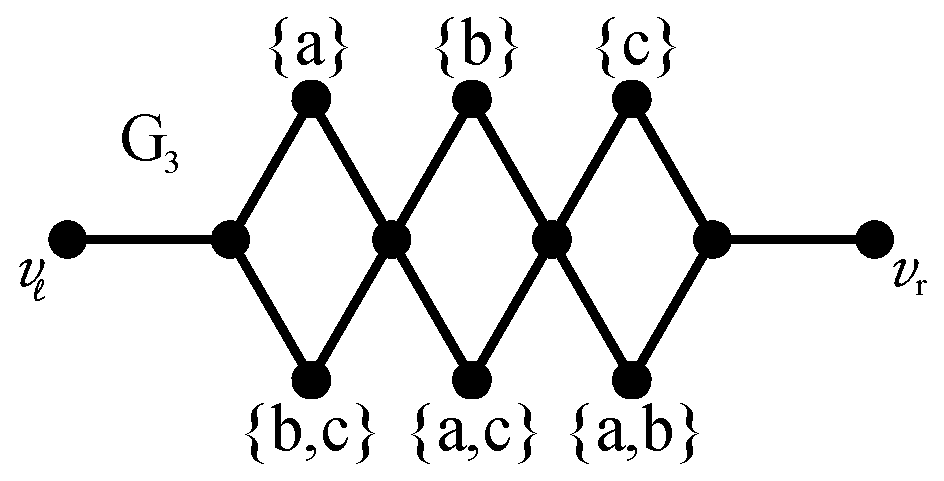
\includegraphics[scale=0.4]{figures/eps/tight-mapexample}
    \caption{An example of the $\mathsf{r}$ map for $G_3$. The set next to
    each top and bottom vertex $u$ is the set $s$ such that $\mathsf{r}(s)=u$.}
    \label{fig:mapexample}
  \end{figure}
  
  We now show that for each $s\in S$, $s=Q\cap\mathcal{T}_{\mathsf{r}(s)}$. This
  is easy to see as $\mathsf{r}(s)$ is internal to all paths in $s$, by
  definition of $\mathsf{r}(s)$ and of the paths in $Q$. On the other end, no
  path from $\mathsf{c}(s)$ goes through $\mathsf{r}(s)$ because it goes through
  the corresponding vertex of $\mathsf{r}(s)$ (top if $\mathsf{r}(s)$ is a
  bottom vertex, bottom otherwise). It is also straightforward to see that,
  if we let $v_Q$ be any arbitrary middle vertex different from $v_\ell$
  or $v_\mathrm{r}$, we have $Q=Q\cap\mathcal{T}_{v_Q}$, given that all paths in
  $Q$ go through all the middle vertices. Also, given that $v_\ell$ is not
  internal to any path, we have $\emptyset=Q\cap\mathcal{T}_{v_\ell}$. Then all
  subsets of $Q$ can be expressed as the intersection between $Q$ and a range
  from $\range_{G_d}$, which means that $Q$ can be shattered and therefore
  $\VC(\range_{G_d})\ge d$.

  From Lemma~\ref{lem:vcdimuppbound} we know that $\VC(\range_{G_d})\le d$, so
  it must be $\VC(\range_{G_d})=d$.
%\end{IEEEproof} 
\end{proof}
\else
Due to space constraints, we defer the proof to the extended online version of
the paper~\citep{RiondatoK13}.
\fi

\begin{figure}[th]
  \centering
  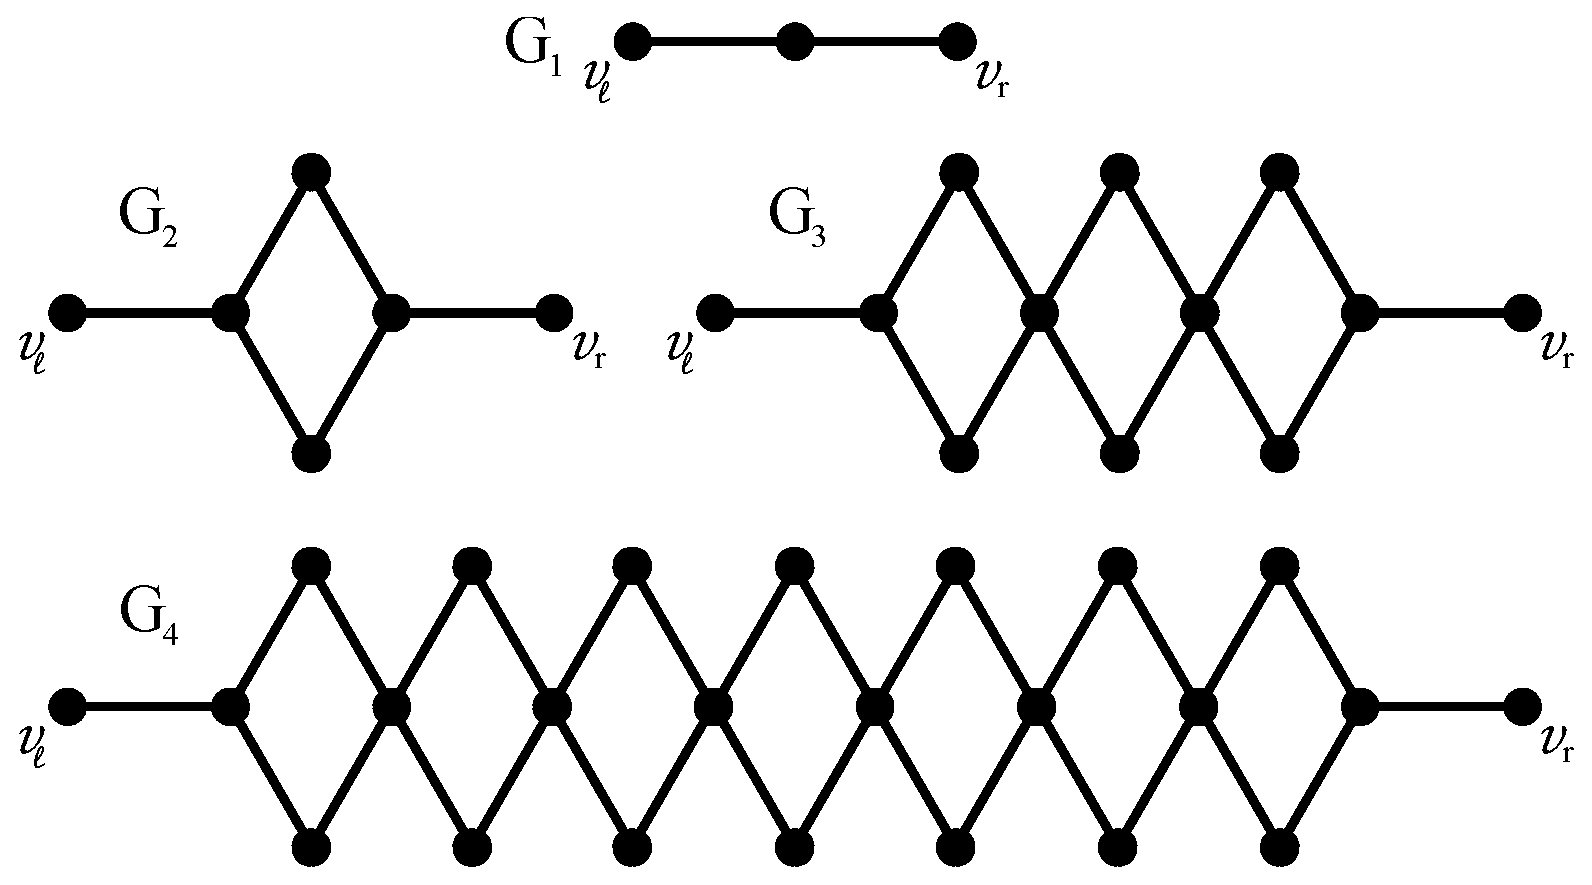
\includegraphics[scale=0.3]{figures/eps/tight}
  \caption{Examples of concertina graphs $G_d$ for $d=1,2,3,4$.}
  \label{fig:tightgraphs}
\end{figure}

The upper bound presented in Lemma~\ref{lem:vcdimuppboundunique}  for the case
of unique shortest paths is also strict in the same sense.
\ifproof
\else
The proof can be found in the extended online version of the
paper~\citep{RiondatoK13}.
\fi

\begin{lemma}\label{lem:vcdimlowboundunique}
  There is a graph $G=(V,E)$ with $|\mathcal{S}_{uv}|\le1$ for all
  pairs $(u,v)\in V\times V$ such that the range set $\range_G$ associated to the
  shortest paths in $G$ has VC-Dimension exactly $3$.
\end{lemma}

\ifproof
\begin{figure}[ht]
  \centering
  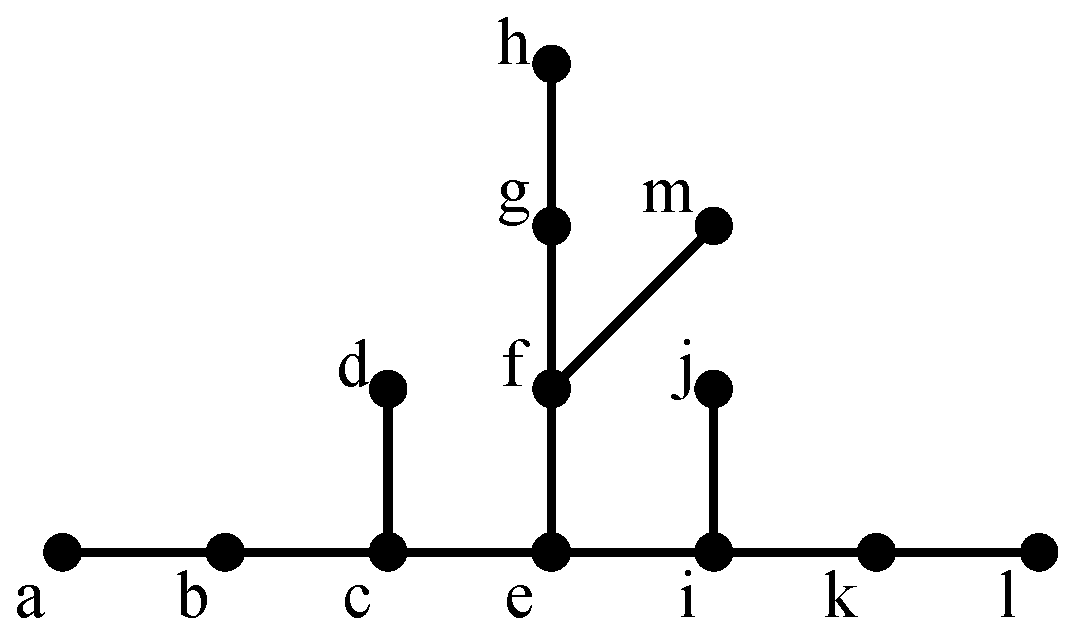
\includegraphics[scale=0.35]{figures/eps/uniqueshortestpathtight}
  \caption{Graph $G$ with $\VC(\range_G)= 3$.}
  \label{fig:uniquetight}
\end{figure}

\begin{proof}
%\begin{IEEEproof}
  Consider the graph $G$ in Fig.~\ref{fig:uniquetight}.
  Let $p_1=(a,b,c,e,i,j)$, $p_2=(m,f,e,i,k,l)$, $p_3=(d,c,e,f,g,h)$ be three
  paths. We now show that $Q=\{p_1,p_2,p_3\}$ can be shattered by $\range_G$, which
  implies $\VC(\range_G)\ge 3$. We have $\emptyset=Q\cap\mathcal{T}_a$,
  $\{p_1\}=Q\cap\mathcal{T}_b$, $\{p_2\}=Q\cap\mathcal{T}_k$,
  $\{p_3\}=Q\cap\mathcal{T}_g$, $\{p_1,p_2\}=Q\cap\mathcal{T}_i$,
  $\{p_1,p_3\}=Q\cap\mathcal{T}_c$, $\{p_2,p_3\}=Q\cap\mathcal{T}_f$,
  $\{p_1,p_2,p_3\}=Q\cap\mathcal{T}_e$,  
  Hence all subsets of $Q$ can be expressed as the intersection between $Q$ and
  some range in $\range_G$ which means that $Q$ can be shattered and
  $\VC(\range_G)\ge 3$. Lemma~\ref{lem:vcdimuppboundunique} gives us an upper
  bound $\VC(\range_G)\le3$, so we can conclude that $\VC(\range_G)=3$.
%\end{IEEEproof}
\end{proof}
\fi

\section{Algorithms}\label{sec:algo}
In this section we present our algorithms to compute a set of approximations for the
betweenness centrality of the (top-$K$) vertices in a graph through sampling,
with probabilistic guarantees on the quality of the approximations.

\subsection{Approximation for all the vertices}\label{sec:allvertapprox}
The intuition behind the algorithm to approximate the betweenness values of all
vertices is the following. Given a graph $G=(V,E)$
with vertex-diameter $\VD(G)$ and two parameters $\varepsilon,\delta\in(0,1)$
we first compute a sample size $r$ using~\eqref{eq:vceapprox} with
\[d=\lfloor\log_2(\VD(G)-2)\rfloor+1\enspace.\]
The resulting sample size is
\begin{equation}\label{eq:samplesize}
r=\frac{c}{\varepsilon^2}\left(\lfloor\log_2(\VD(G)-2)\rfloor+1+\ln\frac{1}{\delta}\right)\enspace.
\end{equation}
This is sufficient to achieve the desired accuracy
(expressed through $\varepsilon$) with the desired confidence (expressed through
$1-\delta$). The algorithm repeats the following steps $r$ times:
\emph{1.}~it samples a pair $u,v$ of distinct vertices uniformly at random,
\emph{2.}~it
computes the set $\mathcal{S}_{uv}$ of all shortest paths between $u$ and $v$,
\emph{3.}~it selects a path $p$ from $\mathcal{S}_{uv}$ uniformly at random,
\emph{4.}~it increases by $1/r$ the betweenness estimation of each vertex in
$\mathsf{Int}(p)$. Note that if the sampled vertices $u$ and $v$ are not
connected, we can skip steps 3 and 4 because we defined
$\mathcal{S}_{uv}=\{p_\emptyset\}$. Denoting with $S$ the set of the sampled
shortest paths, the \emph{unbiased} estimator $\tilde\betw(w)$ for the betweenness
$\betw(w)$ of a vertex $w$ is the sample average 
\[
\tilde\betw(w) = \frac{1}{r}\sum_{p\in S}
\mathds{1}_{\mathsf{Int}(p)}(w) = \frac{1}{r}\sum_{p\in S}
\mathds{1}_{\mathcal{T}_w}(p)\enspace.
\]

There are two crucial steps in this algorithm: the computation of $\VD(G)$ and
the sampling of a path uniformly at random from $\mathcal{S}_{uv}$. We first
deal with the latter, and then present a linear-time constant-factor approximation algorithm for $\VD(G)$.
%in Sect.~\ref{sec:diam}. 
Algorithm~\ref{alg:algorithm} presents the pseudocode of the algorithm,
including the steps to select a random path.  The
\texttt{computeAllShortestPaths(}$u,v$\texttt{)}  on
line~\ref{algline:shortestpaths} is a call to a modified Dijkstra's (or BFS)
algorithm to compute the set $\mathcal{S}_{uv}$, with the same modifications
as~\citep{Brandes01}. The \texttt{getDiameterApprox()} procedure computes an approximation for $\VD(G)$. % (see Sect.~\ref{sec:diam} for details).

\paragraph{Unique shortest paths} 
When, for each pair $(u,v)$ of vertices of $G$, either there is a unique
shortest path from $u$ to $v$ or $v$ is unreachable from $u$, 
%When each pair $(u,v)$ of vertices of $G$ has a unique shortest path connecting them or
%When there is an unique shortest
%path between each pair of vertices of $G$, 
 then one can apply Lemma~\ref{lem:vcdimuppboundunique} and obtain a smaller
sample size
\[
  r= \frac{c}{\varepsilon^2}\left(3+\ln\frac{1}{\delta}\right)
\]
to approximate the betweenness values of all the vertices. 
This is an interesting result: the number of samples needed to compute a good
approximation to all vertices is a \emph{constant} and completely
\emph{independent from $G$}. Intuitively, this means that the algorithm is
extremely fast on graphs with this property. Unique shortest paths are common or
even enforced in road networks by slightly perturbing the edge weights or having
a deterministic tie breaking policy~\citep{GeisbergerSS08}.

\ifproof
\else
\paragraph{Bounded-distance betweenness} For the case of
$k$-bounded-distance betweenness, the sample size on line~\ref{algline:forloop}
of Alg.~\ref{alg:algorithm} can be reduced to 
\[ 
  r= \frac{c}{\varepsilon^2}\left(\lfloor\log_2(k-1)\rfloor + 1 +\ln\frac{1}{\delta}\right)
\]
and the computation of the shortest paths on line~\ref{algline:shortestpaths}
can be stopped after we reached the vertices that are $k$ ``hops'' far from $u$.
\fi

\paragraph{Sampling a shortest path}
Our procedure to select a random shortest path from $\mathcal{S}_{uv}$ is
inspired by the dependencies accumulation procedure used in Brandes' exact
algorithm~\citep{Brandes01}. 
%Given a vertex $w$, ~\citet{Brandes01} showed how
%to compute, for every vertex $z$, the amount $\sigma_{wz}$ of shortest paths
%from $w$ to $z$, while computing the set $\mathcal{S}_{wz}$. 
Let $u$ and $v$ be the vertices sampled by our algorithm
(Step~\ref{algline:samplevertices} of Alg.~\ref{alg:algorithm}). We assume that $u$ and
$v$ are connected otherwise the only possibility is to select the empty path
$p_\emptyset$. Let $y$ be any vertex belonging to at least one shortest path
from $u$ to $v$. Following~\citet{Brandes01}, we can compute $\sigma_{uy}$ and
$\mathcal{S}_{uy}$ while we compute the set $\mathcal{S}_{uv}$ of all the
shortest paths from $u$ to $v$. We can then use this information to select a
shortest path $p$ uniformly at random from $\mathcal{S}_{uv}$ as follows. For each vertex
$w$ let $P_u(w)$ be the subset of neighbors of $w$ that are \emph{predecessors}
of $w$ along the shortest paths from $u$ to $w$. Let $p^*=\{v\}$. Starting from
$v$, we select one of its predecessors $z\in P_u(v)$ using weighted random
sampling: each $z\in P_u(v)$ has probability $\sigma_{uz}/\sum_{w\in
P_u(v)}\sigma_{uw}$ of being sampled. We add $z$ to $p^*$ and then repeat the
procedure for $z$. That is, we select one of $z$'s predecessors from $P_u(z)$
using weighted sampling and add it to $p^*$, and so on until we reach $u$. Note
that we can update the estimation of the betweenness of the internal vertices
along $p^*$ (the only ones for which the estimation is updated) as we compute
$p^*$.

\begin{lemma}\label{lem:samplpath}
  The path $p^*$ built according to the above procedure is selected uniformly at
  random among the paths in $\mathcal{S}_{uv}$.
\end{lemma}

\begin{proof}
%\begin{IEEEproof}
  The probability of sampling $p^*=(u,z_1,\dotsc,z_{|p^*|-2},v)$ equals to the
  product of the probabilities of sampling the vertices internal to $p^*$, hence
  \[
  \Pr(p^*)=\frac{\sigma_{uz_{|p^*|-2}}}{\sigma_{uv}}\frac{\sigma_{uz_{|p^*|-3}}}{\sigma_{uz_{|p^*|-2}}}\dotsb
  \frac{1}{\sigma_{uz_2}}=\frac{1}{\sigma_{uv}}
  \]
  where we used \citep[Lemma3]{Brandes01} which tells us that for $w\neq u$,
  \[
  \sigma_{uw}=\sum_{j\in P_u(w)}\sigma_{uj}
  \]
  and the fact that for $z_1$, which is a neighbor of $u$, $\sigma_{uz_1}=1$.
%\end{IEEEproof}
\end{proof}

\begin{algorithm}[ht]
  \SetKwInOut{Input}{Input}
  \SetKwInOut{Output}{Output}
  \SetKwComment{Comment}{//}{}
  \SetKwFunction{VertexDiameter}{getVertexDiameter}
  \SetKwFunction{SamplePair}{sampleUniformVertexPair}
  \SetKwFunction{SampleUniform}{sampleUniformPath}
  \SetKwFunction{PairShortestPaths}{computeAllShortestPaths}
   \DontPrintSemicolon
  %\dontprintsemicolon
  \Input{Graph $G=(V,E)$ with $|V|=n$, $\varepsilon,\delta\in(0,1)$}
  \Output{A set of approximations of the betweenness centrality of the vertices
  in $V$}
  \ForEach{$w\in V$}
  {
  $\tilde\betw(v)\leftarrow 0$
  }
  $\VD(G)\leftarrow$\VertexDiameter{G}\label{alg:diamcomp}\; 
  $r\leftarrow (c/\varepsilon^2)(\lfloor\log_2(\VD(G)-2)\rfloor+\ln(1/\delta))$\;
  \For{$i\leftarrow 1$ to $r$}
  {\label{algline:forloop}
  $(u,v)\leftarrow$\SamplePair{$V$}\label{algline:samplevertices}\;
  $\mathcal{S}_{uv}\leftarrow$\PairShortestPaths{$u,v$}\label{algline:shortestpaths}\;
  \If{$\mathcal{S}_{uv}\neq\{p_\emptyset\}$}
  {
  \Comment{Random path sampling and estimation update}
  $j\leftarrow v$\;
  $s\leftarrow v$\;
  $t\leftarrow v$\;
  \While{$t \neq u$} {
  sample $z\in P_s(t)$ with probability $\sigma_{uz}/\sigma_{us}$\;
  \If{$z\neq u$} {
  $\tilde\betw(z) \leftarrow \tilde\betw(z)+1/r$\;
  $s\leftarrow t$\;
  $t\leftarrow z$\;
  }
  }
  }
  } % end For
  \Return{$\{(v,\tilde\betw(v)), v\in V\}$}
  \caption{Computes approximations $\tilde\betw(v)$ of the betweenness
  centrality $\betw(v)$ for all vertices $v\in V$.}
  \label{alg:algorithm}
\end{algorithm}

\paragraph{Approximating the vertex-diameter}%\label{sec:diam}
The algorithm presented in the previous section requires the value of the
vertex-diameter $\VD(G)$ of the graph $G$ (line
\ref{alg:diamcomp} of Alg.~\ref{alg:algorithm}). 
Computing the exact value of $\VD(G)$ could be done by solving the All Pair
Shortest Paths (APSP) problem, and taking the shortest path with the maximum size.
Algorithms for exactly solving APSP problem such as Johnson's which runs in
$O(V^2\log V+VE)$ or Floyd-Warshall's ($\Theta(V^3)$), would defeat our
purposes: once we have all the shortest paths for the computation of
the diameter, we could as well compute the betweenness of all the vertices exactly. 
Given that Thm.~\ref{thm:eapprox} (and Thm.~\ref{thm:releapprox})  only
requires an upper bound to the VC-dimension of the range set, an approximation
of the vertex-diameter would be sufficient for our purposes. Several refined
algorithms for approximating the diameter are
known~\citep{AingwordCIM99,BoitmanisFL06,RodittyW12}, with various running times
and quality of approximations. We briefly present a well-known and simple
approximation algorithm that has the right balance of accuracy and speed
for our purposes.

Let $G=(V,E)$ be an \emph{undirected} graph where \emph{all the edge weights are
equal}.
It is a well-known result that one can obtain a $2$-approximation
$\widetilde\VD(G)$ of the vertex-diameter $\VD(G)$ of $G$ in time $O(V+E)$ in
the following way: 1.~select a vertex $v\in V$ uniformly at random, 2.~compute
the shortest paths from $v$ to all other vertices in $V$, and 3.~finally take
$\widetilde\VD(G)$ to be the sum of the lengths of the two shortest paths with
maximum size (which equals to the two longest shortest paths) from $v$ to two
distinct other nodes $u$ and $w$. 
\ifproof
The approximation guarantee follows from the next lemma.

\begin{lemma}\label{lem:diam}
  $\VD(G)\le\widetilde\VD(G)\le 2\VD(G)$.
\end{lemma}
\begin{proof}
%\begin{IEEEproof}
  Let $v\in V$ be a vertex that we choose uniformly at random from the set $V$.
  Let also $u,w\in V$ be the two vertices such that the sum of the sizes of the
  shortest paths $p_{vu}$ and $p_{vw}$ is maximized among all the shortest paths
  that have $v$ as a source.  We have $\widetilde\VD(G)\le 2\VD(G)$ because
  $|p_{vu}|,|p_{vw}|\le\VD(G)$, so $|p_{vu}|+|p_{vw}|\le 2\VD(G)$. To see
  that $\widetilde\VD(G)\ge\VD(G)$, consider a pair of vertices $x$ and $z$ such
  that the length of a shortest path between $x$ and $z$ is equal to $\VD(G)$.
  Let $p_{xv}$ be a shortest path between $x$ and $v$ and let $p_{vz}$ be a
  shortest path between $v$ and $z$. 
  From the properties of the shortest paths $p_{vu}$, $p_{vw}$ we have
  $|p_{vu}|+|p_{vw}|\geq |p_{vx}|+|p_{vz}|$. Since the graph is undirected
  $|p_{s,t}|=|p_{t,s}|$ for every $s,t\in V$.
  Therefore:
  \[
    \widetilde\VD(G) = |p_{vu}|+|p_{vw}|\geq |p_{vx}|+|p_{vz}| =
    |p_{xv}|+|p_{vz}|\ge\VD(G)\enspace. 
  \]
  For the last inequality we used the fact that since $\VD(G)$ is the size of
  the shortest path from $x$ to $z$, then every other path (in this case
  $p'_{xz}$ which is the merge of $p_{xv}$ and $p_{vz}$) has greater or equal
  length from $p_{x,z}$.
  %$\qed$
%\end{IEEEproof}
\end{proof}
\fi
In case we have multiple connected components in $G$, we compute an upper bound
to the vertex diameter of each component separately by running the above
algorithm on each component, and then taking the maximum. 
The connected components can be computed in $O(n+m)$ by traversing the graph in
a Breadth-First-Search (BFS) fashion starting from a random $v$.
%Let $\tilde\Delta_{G_{1}},\tilde\Delta_{G_{2}}, \ldots , \tilde\Delta_{G_{k}}$
%be the approximations of the diameter for each of the $k$ connected components
%of $G$ as if they were separate graphs.
%The output of the approximation for the graph $G$, is the maximum of the values
%$\tilde\Delta_{G_{1}},\tilde\Delta_{G_{2}}, \ldots , \tilde\Delta_{G_{k}}$.
The time complexity of the approximation algorithm in the case of multiple
connected components is again $O(n+m)$ since the sum of the vertices of
individual components is $n$ and the sum of edges is $m$. 

The use of the above $2$-approximation in the computation of the
sample size from line~\ref{algline:forloop} of Alg.~\ref{alg:algorithm} results
in at most $c/\varepsilon^2$ additional samples than if we
used the exact value $\VD(G)$. The computation of $\widetilde\VD(G)$
does not affect the running time of our algorithm: for the construction of
the first sample we can reuse the shortest paths from the sampled
vertex $v$ that we used to obtain the approximation. Specifically, we can sample
a new vertex $u\neq v$ and then choose with uniform probability one of the
(already computed) shortest paths between $v$ and $u$.

If the graph is directed and/or not all edge weights are equal, the computation
of a good approximation to $\VD(G)$ becomes more problematic. In particular,
notice that there is no relationship between $\VD(G)$ and $\mathsf{diam}(G)$
when $G$ is weighted, as the shortest path with maximum size may not be the
shortest path with maximum weight. In these cases, one can use the size (number
of vertices) of the largest Weakly Connected Component (WCC), as a loose upper
bound to $\VD(G)$. The WCC's can again be computed in $O(n+m)$ using BFS.  This
quantity can be as high as $n$ but for the computation of the sample size we use
its logarithm, mitigating the crudeness of the bound. In this case our sample
size is comparable to that proposed by~\citet{BrandesP07}. %when there is a
%single WCC, as it would depend on $\log n$,
Nevertheless the amount of work done per sample by our algorithm is still much
smaller (see Sect.~\ref{sec:discussion} and~\ref{sec:exper} for more
details). In practice, it is possible that the nature of the network suggests a
much better upper bound to the vertex-diameter of the graph, resulting in a
smaller sample size. %than what suggested by the worst case we just presented.  

\paragraph{Analysis}\label{sec:analysis}
%The algorithm we described and presented in 
Algorithm~\ref{alg:algorithm} offers
probabilistic guarantees on the quality of all approximations of the betweenness
centrality.
\begin{lemma}\label{lem:correctness}
  With probability at least $1-\delta$, all the approximations computed by the
  algorithm are within $\varepsilon$ from their real value:
  \[
  \Pr\left(\exists v\in V \mbox{ s.t. }
  |\betw(v)-\tilde\betw(v)|>\varepsilon\right)<\delta\enspace .
  \]
\end{lemma}

\begin{proof}
%\begin{IEEEproof}
  For each $p_{uv}\in\mathbb{S}_G$ let
  \[
  \pi_G(p_{uv})=\frac{1}{n(n-1)}\frac{1}{\sigma_{uv}}\enspace.
  \]
  It is easy to see that $\pi_G$ is a probability distribution and
  $\pi_G(p_{uv})$ is the probability of sampling the path $p_{uv}$ during an
  execution of the loop on line~\ref{algline:forloop} in
  Alg.~\ref{alg:algorithm}, given the way that the vertices $u$ and $v$ are
  selected and Lemma~\ref{lem:samplpath}.
  
  Consider the range set $\range_G$ and the probability distribution $\prob_G$.
  Let $S$ be the set of paths sampled during the execution of the algorithm.
  For $r$ as in~\eqref{eq:samplesize}, Thm.~\ref{thm:eapprox} tells us that the sample $S$ is a
  $\varepsilon$-approximation to $(\range_G,\prob_G)$ with probability at least
  $1-\delta$. Suppose that this is indeed the case, then from
  Def.~\ref{def:eapprox} and the definition of $\range_G$ we have that
  \[
  \left|\prob_G(\mathcal{T}_v) - \frac{1}{r}\sum_{p\in
  S}\mathds{1}_{\mathcal{T}_v}(p)\right|=\left|\prob_G(\mathcal{T}_v) -
  \tilde\betw(v)\right|\le\varepsilon, \forall v\in
  V\enspace.
  \]
  From the definition of $\prob_G$ we have
  \[
  \prob_G(\mathcal{T}_v)=\frac{1}{n(n-1)}\sum_{p_{uw}\in\mathcal{T}_v}\frac{1}{\sigma_{uw}}=\betw(v),
  \]
  which concludes the proof.
%\end{IEEEproof}
\end{proof}

\ifproof
\paragraph{Time and space complexity.} Clearly the runtime of the algorithm is
dominated by the computation of the shortest path at each step, which takes time
$O(|V|+|M|)$ if the graph is unweighted (BFS algorithm) and time
$O(|E|+|V|\log|V|)$ otherwise (Dijkstra's algorithm with Fibonacci heap).
This time must then be multiplied by $r$ as in~\eqref{eq:samplesize} to obtain
the final time complexity. The space requirements are dominated by the amount of
memory needed to store the graph, so they are either $O(|V|^2)$ if using an
adjacency matrix, or $O(|V|+|E|)$ if using $|V|$ adjacency lists.
\fi

\subsection{High-quality approximation of the top-$K$ betweenness
vertices}\label{sec:topk}
%\XXX It would be great to look at the paper by Ezra, ``Small-Size Relative
%$(p,\varepsilon)$-Approximations for Well-Behaved Range Spaces'', 2012,
%available on the arXiv. She presents a smaller bound to the sample size for a
%relative $(p,\varepsilon$-approximation if the range set is ``well-behaved''. We
%should check whether ours is. (Warning: the paper is not exactly an example of
%clarity\ldots)

Very often in practice one is interested only in identifying the vertices with
the highest betweenness centrality, as they are the ``primary actors'' in the
network. We present here an algorithm to compute a very high-quality
approximation of the set $\TOPK(K,G)$ of the top-$K$ betweenness vertices in a graph
$G=(V,E)$. Formally, let $v_1,\dotsc,v_n$ be a labelling of the vertices in $V$
such that $\betw(v_i)\ge\betw(v_j)$ for $1\le i<j\le n$. Then $\TOPK(K,G)$ is
defined as the set of vertices with betweenness at least $\betw(v_K)$:
\[
\TOPK(K,G)=\{(v,\betw(v)), ~:~ v\in V \mbox{ and } \betw(v)\ge\betw(v_K)\}\enspace.
\]
Note that $\TOPK(K,G)$ may contain more than $K$ vertices. 
%This is in line with
%the definition of the set of top-$k$ Frequent Itemsets in the market basket
%analysis setting \XXX add reference.

Our algorithm works in two phases. Each phase is basically a run of the
algorithm for approximating the betweenness of all vertices. %presented in the previous section. 
The two phases differ in the way they compute the number of paths to sample and
the additional operations at the end of each phase. In the first
phase, we compute a lower bound $\ell'$ to $\betw(v_K)$. In the second phase we
use $\ell'$ to compute the number of samples $r$ needed to obtain a relative
$(\ell',\varepsilon)$-approximation to $(\range_G,\pi_G)$. We use $r$ samples to approximate the betweenness of all vertices again, and
return a collection of vertices that is, with high probability, a superset of
$\TOPK(K,G)$.

Let $\widetilde\VD(G)$ be an upper bound to the vertex-diameter of $G$. Given
$\varepsilon,\delta\in(0,1)$, let $\delta',\delta''$ be two positive reals such
that $(1-\delta')(1-\delta'')\ge(1-\delta)$. Let
\[
r'=\frac{c}{\varepsilon^2}\left(\lfloor\log_2(\widetilde\VD(G)-2)\rfloor+1+\log\frac{1}{\delta'}\right)\enspace.
\]
Let $\tilde\betw'_k$ be the $K$-th highest estimated betweenness obtained using
Algorithm~\ref{alg:algorithm} where $r=r'$, and let
%\[
  $\ell'=\tilde\betw_K-\varepsilon$, %.
%\]
%Let
and
\[
r''=\frac{c'}{\varepsilon^2\ell'}\left((\lfloor\log_2(\widetilde\VD(G)-2)\rfloor+1)\log\frac{1}{\ell'}+\log\frac{1}{\delta''}\right)\enspace.
\]
We run Algorithm~\ref{alg:algorithm} with $r=r''$ and let $\tilde\betw''_K$ be
the so-obtained $K$-th highest estimated betweenness. Let
$\ell''=\min\{\tilde\betw''(v) / (1+\varepsilon) ~:~ v\in V \mbox{ s.t. }
\tilde\betw''(v)\ge\tilde\betw''_K\}$. We
return the collection $\widetilde\TOPK(K,G)$ of vertices $v$ such that
$\tilde\betw''(v)*(1+\varepsilon)/(1-\varepsilon)\ge\ell''$:
\[
\widetilde\TOPK(K,G)= \left\{v\in V ~:~
\tilde\betw''(v)\frac{1+\varepsilon}{1-\varepsilon}\ge\ell''\right\}\enspace.
\]
\ifproof
The pseudocode of the algorithm is presented in Algorithm~\ref{alg:topk}.

\begin{algorithm}[ht]
  \SetKwInOut{Input}{Input}
  \SetKwInOut{Output}{Output}
  \SetKwComment{Comment}{//}{}
  \SetKwFunction{VertexDiameter}{getVertexDiameter}
  \SetKwFunction{SamplePair}{sampleUniformVertexPair}
  \SetKwFunction{SampleUniform}{sampleUniformPath}
  \SetKwFunction{PairShortestPaths}{computeAllShortestPaths}
   \DontPrintSemicolon
  %\dontprintsemicolon
  \Input{a graph $G=(V,E)$ with $|V|=n$, a positive integer $K\le n$, real
  values $\varepsilon,\delta\in(0,1)$}
  \Output{a superset of $\TOPK(K,G)$, with high-quality estimation of the
  betweenness for the vertices in the returned set.}
  $\delta',\delta''\leftarrow$ two positive reals such that
  $(1-\delta')(1-\delta'')\ge(1-\delta)$\;
  $\widetilde\VD(G)\leftarrow$ upper bound to $\VD(G)$\;
  \Comment{First phase}
  $r'\leftarrow\frac{c}{\varepsilon^2}\left(\lfloor\log_2(\widetilde\VD(G)-2)\rfloor+1+\log\frac{1}{\delta''}\right)$\;
  $B'=\{(v,\tilde\betw'(v)) ~:~ v\in V\}\leftarrow$ output of Algorithm~\ref{alg:algorithm} with $r=r'$\;
  $\tilde\betw_K'\leftarrow$ $K$-th highest betweenness value from $B'$, ties
  broken arbitrarily\;
  $\ell'\leftarrow\tilde\betw_K'-\varepsilon$\;
  $r''\leftarrow\frac{c'}{\varepsilon^2\ell'}\left((\lfloor\log_2(\widetilde\VD(G)-2)\rfloor+1)\log\frac{1}{\ell'}+\log\frac{1}{\delta''}\right)$\;
  \Comment{Second phase}
  $B''=\{(v,\tilde\betw''(v)) ~:~ v\in V\}\leftarrow$ output of
  Algorithm~\ref{alg:algorithm} with $r=r''$\;
  $\tilde\betw_K''\leftarrow$ $K$-th highest betweenness value from $B''$, ties
  broken arbitrarily\;
  $\ell''\leftarrow\min\{\tilde\betw''(v)/(1+\varepsilon) ~:~ v \mbox{ s.t. }
  \tilde\betw''(v)\ge\tilde\betw_K''\}$\;
  \Return $\{(v,\tilde\betw''(v)) ~:~ v\in V \mbox{ s.t. }
  \tilde\betw''(v)\frac{1+\varepsilon}{1-\varepsilon}\ge\ell''\}$\;
  \caption{High-quality approximation of the top-$K$ betweenness vertices}
  \label{alg:topk}
\end{algorithm}

\paragraph{Analysis}
The following lemma shows the properties of the collection $\widetilde\TOPK(K,G)$.
\fi

\begin{lemma}
  With probability at least $1-\delta$, 
  \begin{enumerate*}
    \item $\TOPK(K,G)\subseteq \widetilde\TOPK(K,G)$, and
    \item for all $v\in\TOPK(K,G)$ we have
      $|\tilde\betw''(v)-\betw(v)|\le\varepsilon\betw(v)$, and
    \item no vertex $u\in\widetilde\TOPK(K,G)\setminus\TOPK(K,G)$ has an estimated
      betweenness greater than $\ell'(1+\varepsilon)$.
  \end{enumerate*}
\end{lemma}
\ifproof
\begin{proof}
%\begin{IEEEproof}
  We start by proving 1. From Thm.~\ref{thm:eapprox} we know that, with probability at least
  $1-\delta'$, a sample of size $r'$ is a $\varepsilon$-approximation to
  $(\range_G,\pi_G)$ and from Thm.~\ref{thm:releapprox} we have that with
  probability at least $1-\delta''$ a sample of size $r''$ is a relative
  $(\ell',\varepsilon)$-approximation to $(\range_G,\pi_G)$. Suppose both these
  events occur, which happens with probability at least $1-\delta$. Then it is
  easy to see that $\ell'\le\betw(v_K)$, as there must be at least $K$ vertices
  with exact betweenness greater or equal to $\ell'$.  Consider now $\ell''$.
  Following the same reasoning as for $\ell'$, it should be clear that
  $\ell''\le\betw(v_K)$. The vertices included in $\widetilde\TOPK(K,G)$ are all and
  only those vertices that \emph{may} have exact betweenness at least $\ell''$,
  which implies that all vertices that have exact betweenness at least
  $\betw(v_K)$ are included in $\widetilde\TOPK(K,G)$. 
  Points 2 and 3 in the thesis follow from the properties of the relative
  $(\ell',\varepsilon)$-approximation (Def.~\ref{def:releapprox}).
%\end{IEEEproof}
\end{proof}
\else
We refer the reader interested in the proof to the extended online version of
the paper~\citep{RiondatoK13}.
\fi

The advantage of using our algorithm to approximate the collection of top-$K$
betweenness vertices consists in the very high-quality approximation of the
betweenness values for the returned set of vertices: they are all within a
multiplicative factor $\varepsilon$ from their exact values. By reverse-sorting
them according to the approximated betweenness, one can obtain a ranking that is
very similar to the original exact one. Previous algorithms could not achieve such a
good ranking as they were only able to approximate the betweenness values to
within an additive error $\varepsilon$. The cost of computing the high quality
approximation for the top-$K$ vertices is the cost of an additional run of our
algorithm to compute good approximations for all the vertices.

\subsection{Discussion}\label{sec:discussion}
\citet{JacobKLPT05} and independently~\citet{BrandesP07} present a
sampling-based algorithm to approximate the betweenness centrality of all the
vertices of the graph. The algorithm (which we call \textsf{BP}) creates a
sample $S=\{v_1,\dotsc,v_r\}$ of $r$ vertices drawn uniformly at random and
computes all the shortest paths between each $v_i$ to all other vertices in the
graph. Their estimation $\tilde\betw_\mathsf{BP}(u)$ for $\betw(u)$ is
\[ 
\tilde\betw_\mathsf{BP}(u)= \frac{1}{(n-1)r}\sum_{v_i\in S}\sum_{\substack{w\neq
v_i\\w\neq
u}}\sum_{p\in\mathcal{S}_{v_iw}}\frac{\mathds{1}_{\mathsf{Int}(p)}(u)}{|\mathcal{S}_{v_iw}|}\enspace.
\]
As it was for Algorithm~\ref{alg:algorithm}, the key ingredient to ensure a correct
approximation for the betweenness centrality is the computation of the sample
size $r$. Inspired by the work of~\citet{EppsteinW04}, \citet{BrandesP07} 
%rely
%on the following classical result by~\citet{Hoeffding63} for their computation
%of $r$.
%\begin{theorem}[\citep{Hoeffding63}]
%  Let $X_1,X_2,\dotsc,X_r$ be a sequence of independent random variables
%  such that $a_i\leq X_i\leq b_i$. Then for any $\xi > 0$
%  \begin{align}\label{eq:hoeffding}
%    \begin{split}
%      \Pr&\left(\left|\frac{|\sum_{i=1}^rX_i|}{r}-\mathbf{E}\left[\frac{|\sum_{i=1}^rX_i|}{r}\right]\right|\geq
%    \xi\right)\le \\
%      &\leq 2e^{-2r^2\xi^2/\sum_{i=1}^{r}(b_{i}-a_{i})^2}\enspace.
%    \end{split}
%  \end{align}
%\end{theorem}
%
%\citet{BrandesP07} use this result to compute a sample size $r$ sufficient to ensure that, for
%a fixed vertex $u$,
%\[ 
%\Pr\left(|\betw(u)-\tilde\betw'(u)|>\varepsilon\right)<\frac{\delta}{n}\enspace.
%\]
%In their setting $\xi=\varepsilon$ and there is a variable $X_i$ for
%each vertex $v_i$ in the sample:
%\[ 
%X_i=\frac{1}{n-1}\sum_{w\neq v_i,w\neq
%u}\sum_{p\in\mathcal{S}_{v_iw}}\frac{\mathds{1}_{\mathsf{Int}(p)}(u)}{|\mathcal{S}_{v_iw}|}\enspace
%.
%\]
%It is easy to see that $0\le X_i\le 1$. Moreover,
%\[
%  \mathbf{E}\left[\frac{|\sum_{i=1}^r X_i}{r}\right] = \betw(u)\enspace.
%\]
%%\begin{align*}
%%\mathbf{E}\left[\frac{|X_1+\dotsb+X_r|}{r}\right] &=
%%\frac{1}{r(n-1)}\mathbf{E}\left[\sum_{v_i\in S}\sum_{w\neq v_i,w\neq
%%u}\sum_{p\in\mathcal{S}_{v_iw}}\frac{\mathds{1}_{\mathsf{Int}(p)}(u)}{|\mathcal{S}_{v_iw}|}\right]
%%=\frac{1}{r(n-1)}\sum_{v\in V}\mathbf{E}\left[Y_v\sum_{w\neq v,w\neq
%%u}\sum_{p\in\mathcal{S}_{vw}}\frac{\mathds{1}_{\mathsf{Int}(p)}(u)}{|\mathcal{S}_{vw}|}\right] =
%%\\
%%&=\frac{1}{r(n-1)}\sum_{v\in V}\mathbf{E}[Y_v]\sum_{w\neq v,w\neq
%%u}\sum_{p\in\mathcal{S}_{vw}}\frac{\mathds{1}_{\mathsf{Int}(p)}(u)}{|\mathcal{S}_{vw}|}
%%=\frac{1}{r(n-1)}\sum_{v\in V}\frac{r}{n}\sum_{w\neq v,w\neq
%%u}\sum_{p\in\mathcal{S}_{vw}}\frac{\mathds{1}_{\mathsf{Int}(p)}(u)}{|\mathcal{S}_{vw}|}
%%= \betw(u),
%%\end{align*}
%%where $Y_v$ is a Bernoulli random variable taking value 1 if $v\in S$, and 0
%%otherwise, so $\mathbf{E}[Y_v]=\Pr(Y_v=1)=r/n$.
%Plugging these values in~\eqref{eq:hoeffding}, we have
%\[
%\Pr\left(|\betw(u)-\tilde\betw'(u)|>\varepsilon\right)\leq
%2e^{-2r\epsilon^2}\enspace.
%\]
%We want this probability to be at most $\delta/n$, so we need a sample of size
%They
prove that, to obtain good (within $\varepsilon$) estimations for the
betweenness of all vertices with probability at least $1-\delta$, it must be
\[
r\geq \frac{1}{2\varepsilon^2}\left(\ln n + \ln 2 +\ln\frac{1}{\delta}\right)\enspace.
\]
%An application of the union bound over the $n$ vertices ensures a uniform
%(simultaneous) guarantee on the quality of
%all the estimation, with probability at least $1-\delta$.
From this expression it should be clear that this sample size is usually much
larger than ours, as in practice $\VD(G)\ll n$. For the same reason, this
algorithm would not scale well as the network size increases (see also
Sect.~\ref{sec:exper}).

Another interesting aspect in which our algorithm and \textsf{BP} differ is the
\emph{amount of work done per sample}. Our algorithm computes a single set
$\mathcal{S}_{uv}$ for the sampled pair of vertices $(u,v)$: it performs a run
of Dijkstra's algorithm (or of BFS) from $u$, stopping when $v$ is reached.
\textsf{BP} instead computes all the sets $\mathcal{S}_{uw}$ from the sampled
vertices $u$ to all other vertices, again with a single run of Dijkstra or BFS,
but without the ``early-stopping condition'' that we have when we reach $v$.
Although in the worst case the two computations have the same time
complexity\footnote{It is a well-known open problem whether there is an
algorithm to perform a single $s,t$-shortest path computation between a pair of
vertices with smaller worst-case time complexity than the Single Source Shortest
Path computation.}, in practice we perform many fewer operations, as we can
expect $v$ not to always be very far from $u$ and therefore we can terminate
early. This fact has a huge impact on the running time. Our algorithm also
touches \emph{many fewer} edges than \textsf{BP}. The latter can touch all the
edges in the graph \emph{at every sample}, while our computation exhibits a much
higher \emph{locality}, exploring only a neighborhood of $u$ until $v$ is
reached. The results of our experimental evaluation presented in
Sect.~\ref{sec:exper} highlights this and other advantages of our method over
the one from~\citep{JacobKLPT05,BrandesP07}. In the future, we plan to
investigate the possibility of using \emph{bidirectional A$^*$
search}~\citep{Pohl69,KaindlK97} to further speed up the computation for each
sample of our algorithms.

\ifproof
The analysis of Algorithm 1 allow us to obtain a tighter analysis for the
algorithm by~\citet{BrandesP07} and~\citet{JacobKLPT05}.

\begin{lemma}\label{lem:variance}
  Fix $r>0$ and let $w\in V$. Let $\tilde\betw_\mathsf{BP}(w)$ be the estimation
  of the betweenness $\betw(w)$ computed by \textsf{BP} using $r$ samples, and
  let $\tilde\betw(w)$ be the estimation computed by
  Algorithm~\ref{alg:algorithm} using $r$ samples. The estimator
  $\tilde\betw_\mathsf{BP}(w)$ is \emph{uniformly better} than the estimator
  $\tilde\betw(w)$. I.e., for any value of $\betw(w)$ and $r$, we have
  \[
  \var[\tilde\betw_\mathsf{BP}(w)]\le\var[\tilde\betw(w)]\enspace.
  \]
\end{lemma}

\begin{proof}
  Consider the quantity
  \[
  \var[\tilde\betw(w)]-\var[\tilde\betw_\mathsf{BP}(w)]\enspace.\]
  We will show that the above quantity is greater than or equal to 0, proving
  the thesis.
  Since
  $\exp[\tilde\betw(w)]=\exp[\tilde\betw_\mathsf{BF}(w)]=\betw(w)$
  and using the definition of variance, we only need to show 
  \begin{equation}\label{eq:inequal}
    \exp[(\tilde\betw(w))^2]-\exp[(\tilde\betw_\mathsf{BF}(w))^2]\ge
    0\enspace.
  \end{equation}

  Let start from computing $\exp[(\tilde\betw_\mathsf{BF}(w))^2]$. For every
  vertex $v$, we define $\alpha_v$ as
  \[
  \alpha_v=\frac{1}{n-1}\sum_{\substack{u\in V
  \\u\neq
  v}}\sum_{p\in\mathcal{S}_{vu}}\frac{\mathds{1}_{\mathsf{Int}(p)}(w)}{\sigma_{vu}}\enspace.
  \]
  Note that 
  \begin{equation}\label{eq:betwalpha}
    \betw(w)=\frac{1}{n}\sum_{v\in V}\alpha(v)\enspace.
  \end{equation}
  Consider, for $1\le i \le r$, the contribution $X_i$ to $\tilde\betw_\mathsf{BP}(w)$
  of the paths computed from the $i$\textsuperscript{th} sampled vertex. $X_i$
  is a random variable that takes value $\alpha_v$ with probability $1/n$, for
  all $v\in V$. We have
  \begin{equation}\label{eq:xiexpvar}
    \exp[X_i]=\sum_{v\in V}\frac{1}{n}\alpha_v=\betw(w) \mbox{ and }
    \exp[X_i^2]=\frac{1}{n}\sum_{v\in V}\alpha_v^2, \forall 1\le i\le r\enspace.
  \end{equation}
  Clearly
  \[
  \tilde\betw_\mathsf{BP}(w)=\frac{1}{r}\sum_{i=1}^r X_i\enspace.
  \]
  The variables $X_i$'s are independent and identically distributed so
  \begin{align}\label{eq:expxisquared}
    \exp[(\tilde\betw_\mathsf{BP}(w))^2]&=\frac{1}{r^2}\exp\left[\left(\sum_{i=1}^rX_i\right)^2\right]=\frac{1}{r^2}\sum_{i=1}^r\left(\exp[X_i^2]+\sum_{j=i+1}^r(\exp[X_i]\exp[X_j])\right)=\frac{1}{r}\frac{1}{n}\sum_{v\in
    V}\alpha_v^2+\frac{r-1}{r}(\betw(w))^2,
\end{align}
where we used~\eqref{eq:xiexpvar}.

We now compute $\exp[(\tilde\betw(w))^2]$. 
Consider the contribution $Y_i$ to $\tilde\betw(w)$ of the
$i$\textsuperscript{th} sampled path by Algorithm 1, for $1\le i\le r$. $Y_i$ is a random variable that takes value
$\mathds{1}_{\mathsf{Int}(p)}(w)$ with probability $\pi(p)$, for every shortest
path $p\in\mathbb{S}_G$. We have
\begin{equation}\label{eq:yiexpvar}
  \exp[Y_i]=\exp[Y_i^2]=\betw(w), \forall 1\le i \le r\enspace.
\end{equation}
By definition, 
\[
\tilde\betw(w)=\frac{1}{r}\sum_{i=1}^rY_i\enspace.
\]
The random variables $Y_i$ are independent and identically distributed so
\begin{align}\label{eq:expyisquared}
  \exp[(\tilde\betw(w))^2]&=\frac{1}{r^2}\exp\left[\left(\sum_{i=1}^r
  Y_i\right)^2\right]=\frac{1}{r^2}\sum_{i=1}^r\left(\exp[Y_i^2]+\sum_{j=i+1}^r\exp[Y_i]\exp[Y_j]\right)=\frac{1}{r}\betw(w)+\frac{r-1}{r}(\betw(w))^2,
\end{align}
where we used~\eqref{eq:yiexpvar}.

We can now rewrite the left side of~\eqref{eq:inequal} using
~\eqref{eq:betwalpha},~\eqref{eq:expxisquared},~and~\eqref{eq:expyisquared}:
\begin{align*}
  \exp[(\tilde\betw(w))^2]-\exp[(\tilde\betw_\mathsf{BF}(w))^2] &=
  \frac{1}{r}\betw(w)+\frac{r-1}{r}(\betw(w))^2 - \frac{1}{r}\frac{1}{n}\sum_{v\in
    V}\alpha_v^2
   -\frac{r-1}{r}(\betw(w))^2 =
    \frac{1}{r}\frac{1}{n}\sum_{v\in V}(\alpha_v - \alpha_v^2)\enspace. 
\end{align*}
Since $\alpha_v\in[0,1]$, we have $\alpha_v-\alpha_v^2\ge 0$ for all $v$, and our proof
is complete.
\end{proof}

The following lemma is an easy consequence of the above.

\begin{lemma}\label{lem:MSE}
  \textsf{BP} has lower expected Mean Squared Error than Algorithm~1:
  \[
  \exp[\mse_\mathsf{BP}]\le \exp[\mse]\enspace.
  \]
\end{lemma}

\begin{proof}
  We have
  \[ 
  \exp[\mse_\mathsf{BP}] = \exp\left[\frac{1}{n}\sum_{v\in
  V}\left(\tilde\betw_\mathsf{BP}(w)-\betw(v)\right)^2\right]=\frac{1}{n}\sum_{v\in
  V}\exp\left[\left(\tilde\betw_\mathsf{BP}(w)-\betw(v)\right)^2\right]=\frac{1}{n}\sum_{v\in
  V}\var[\tilde\betw_\mathsf{BP}(w)],
  \]
  where we used the linearity of expectation and the fact that the estimator
  $\tilde\betw_\mathsf{BP}(w)$ is unbiased for $\betw(w)$ ($\exp[\tilde\betw_\mathsf{BP}(w)]=\betw(w)]$).
  Analogously for Algorithm~1:
  \[
  \exp[\mse] = \frac{1}{n}\sum_{v\in V}\var[\tilde\betw(w)]\enspace.
  \]
  Hence
  \[
  \exp[\mse]-\exp[\mse_\mathsf{BP}]=\frac{1}{n}\sum_{v\in
  V}\left(\var[\tilde\betw(w)]-\var[\tilde\betw_\mathsf{BP}(w)]\right),
  \]
  and from Lemma~\ref{lem:variance} we have that each addend of the sum is
  non-negative and so is the above expression, concluding our proof.
\end{proof}

%\begin{lemma}
%  Let $G=(V,E)$ be a graph, and $\varepsilon,\delta\in(0,1)$. Let
%  \[
%  r =
%  \frac{c}{\varepsilon^2}\left(\lfloor\log_2(\mathsf{VD}(G)-2\rfloor+1+\ln\frac{1}{\delta}\right)\enspace.
%  \]
%  and let $S$ be a set of vertices of $G$ sampled uniformly at random with
%  replacement from $V$. Let $\tilde\betw_{\mathsf{BP}}(w)$ be the estimated
%  value for $\betw(w)$ computed by \textsf{BP} using $S$. Then
%  \[
%  \Pr(\exists w\in V \mbox{ s.t. }
%  |\tilde\betw_{\mathsf{BP}}(w)-\betw(w)|>\varepsilon)<\delta\enspace.
%  \]
%  %If Algorithm 1 computes an $(\varepsilon,\delta)$-approximation with $r$
%  %samples, then the algorithm by~\citet{BrandesP07} does the same with the same
%  %number of samples.
%\end{lemma}
%
%\begin{proof}
%  Consider a simple coupling of the executions of Algorithm 1 and \textsf{BP}
%  for $r$ samples: when Algorithm 1 samples a shortest path from a vertex $v$ to a vertex $u$,
%  \textsf{BP} samples the vertex $v$. 
%
%Consider an execution of the algorithms and let $X_v$ be the number of times
%that vertex $v$ is the starting point of a sampled path. 
%
%The estimation for the betweenness of vertex $w$ computed by \textsf{BP} is
%\[
%\tilde\betw_{\mathsf{BP}}(w)=\frac{1}{r}\sum_{v\in V}
%X_v\underbrace{\left(\frac{1}{n-1}\sum_{\substack{u\in V \\u\neq
%v}}\sum_{p\in\mathcal{S}_{vu}}\frac{\mathds{1}_{\mathsf{Int}(p)}(w)}{|\mathcal{S}_{vu}|}\right)}_{Y_v(w)}\enspace.
%\]
%The estimation for the betweenness of vertex $w$ computed by Algorithm 1
%is
%\[
%\tilde\betw_{\mathrm{A1}}(w)=\frac{1}{r}Z_w,
%\]
%where $Z_w$ is the number of times that a path containing the vertex $w$ gets
%sampled. Now, for each $v$ and for $1\le i\le X_v$, let $p_v^{(i)}$ be the path
%sampled the $i$\textsuperscript{th} time that the sampled path had $v$ as
%starting vertex, and let $A_v^{(i)}(w)=1$ if $w\in\mathsf{Int}(p_v^{(i)}$, and
%$A_v^{(i)}(w)=0$ otherwise. Then it is clear that 
%\[
%\tilde\betw_{\mathrm{A1}}(w)=\frac{1}{r}\sum_{v\in V}
%X_v\frac{\sum_{i=1}^{X_v}A^{(i)}_v(w)}{X_v}\enspace.
%\]
%We claim that
%\[
%\mathbb{E}\left[\left.\frac{\sum_{i=1}^{X_v}A^{(i)}_v(w)}{X_v}\right|X_v\right]=Y_v(w),\]
%where the expectation is taken over the choice of the paths, which are sampled
%according to the distribution $\pi$.
%To see this, consider $\mathbb{E}[A_v^{(i)}(w) ~|~ X_v]$. It
%is clear that $A^{(i)}(w)$ and $X_v$ are independent, for $1\le i\le X_v$. From
%this and the definition of expectation we have 
%\[
%\mathbb{E}\left[\left.A_v^{(i)}(w)\right|X_v\right] =
%\mathbb{E}\left[A_v^{(i)}(w)\right]=\frac{1}{n-1}\sum_{\substack{u\in V
%\\u\neq
%v}}\sum_{p\in\mathcal{S}_{vu}}\frac{\mathds{1}_{\mathsf{Int}(p)}(w)}{|\mathcal{S}_{vu}|}
%=Y_v(w)\enspace.
%\]
%This expression does not depend on $i$.
%
%The claim then follows easily from the linearity of expectation:
%\[
%\mathbb{E}\left[\left.\frac{\sum_{i=1}^{X_v}A^{(i)}_v(w)}{X_v}\right|X_v\right] =
%\sum_{i=1}^{X_v}\mathbb{E}\left[\left.\frac{A^{(i)}_v(w)}{X_v}\right|X_v\right]=\sum_{i=1}^{X_v}\frac{1}{X_v}\mathbb{E}\left[A_v^{(i)}(w)\right]=\mathbb{E}\left[A_v^{(1)}(w)\right]=Y_v(w)\enspace.
%\]
%Recall from Lemma~\ref{lem:variance} that the estimator
%$\tilde\betw_{\mathsf{BP}}(w)$ has lower variance than the estimator
%$\tilde\betw(w)$, for all vertices $w$. 
%
%\XXX: The following is not actually true \MR. Since both estimators have
%the same expectation $\betw(w)$, this means that for any $a\in[0,1]$ we have
%\[
%\Pr\left(|\tilde\betw_{\mathsf{BP}}(w)-\betw(w)|>a\right)\le\Pr(\left(|\tilde\betw(w)-\betw(w)|>a\right)\enspace.
%\]
%
%This means that for every collection of $r$ samples for which Algorithm 1 computes estimates
%$\tilde\betw(w)$ such that
%\begin{equation}\label{eq:edapprox}
%|\tilde\betw(w)-\betw(w)|\le\varepsilon, \forall w\in W,
%\end{equation}
%so would \textsf{BP} using the $r$ samples according to the coupling. For
%Algorithm $1$ the event in~\eqref{eq:edapprox} occurs with probability at least
%$1-\delta$ over the choice of samples, and so would be for \textsf{BP},
%concluding our proof.
%\end{proof}
%

The estimator $\tilde\betw_{\mathsf{BP}}(w)$ has lower variance and MSE than
$\tilde\betw(w)$, which means that it can give better estimations of the
betweenness values in practice using the same number of samples. Before always
opting for \textsf{BP} (or for the algorithm by~\citet{GeisbergerSS08}, whose
estimators have even lower variance than those of \textsf{BP}) with a number of
samples equal to the one in~\eqref{eq:samplesize}, one should
nevertheless take into account two facts. Firstly, we do not currently have a
proof that \textsf{BP} (or the algorithm from~\citep{GeisbergerSS08}) can
compute, with a number of samples as in~\eqref{eq:samplesize},
a good (within $\pm\varepsilon$) approximation of the betweenness of all
vertices with probability at least $1-\delta$.\footnote{We conjecture that this
is true and are currently working on a proof.}
Secondly we already argued that per sample, the computation of
$\tilde\betw_{\mathsf{BP}}(w)$ requires more time than the one for
$\tilde\betw_{\mathrm{A1}}(w)$. The difference is even larger if
Algorithm~\ref{alg:algorithm} uses bidirectional
search~\citep{KaindlK97,Pohl69}. 

We can conclude this discussion stating that Algorithm~\ref{alg:algorithm},
\textsf{BP}, and the algorithm by~\citet{GeisbergerSS08} share the same design
principles, but choose different trade-offs between accuracy and speed.  
\fi

\begin{figure*}
  \centering
  \subfloat[Undirected graphs]{
  \begin{small}
    \begin{tabular}{cccccc}
      \toprule
      &  & & &  \multicolumn{2}{c}{$\frac{\mbox{Time}_\mathsf{BP}}{\mbox{Time}_\mathsf{VC}}$} \\
      \cmidrule(r){5-6}
      & \multicolumn{3}{c}{Graph Properties} & \multicolumn{2}{c}{diam-2approx} \\
      \cmidrule(r){2-4} \cmidrule(r){5-6}
      Graph & $|V|$ & $|E|$ & $\VD(G)$ & min & max \\
      \midrule
      oregon1-010331 & 10,670 & 22,002 & 9 & 4.39 & 4.75\\  % [1ex] adds vertical space
      oregon1-010526 & 11,174 & 23,409 & 10 & 4.26 & 4.73 \\
      ca-HepPh & 12,008 & 237,010 & 13 & 3.06 & 3.33\\
      ca-AstroPh & 18,772 & 396,160  & 14 & 3.26 & 3.76\\
      ca-CondMat & 23,133 & 186,936 & 15 & 3.75 & 4.08\\
      email-Enron & 36,692 & 421,578 & 12 & 3.60 & 4.16\\
      \bottomrule
    \end{tabular}
  \end{small}
  \label{tab:expUndir}
  }
\ifproof
 %

\fi
  \subfloat[Directed graphs]{
  \begin{small}
    \begin{tabular}{cccccccc}
      \toprule
      & & & & \multicolumn{4}{c}{$\frac{\mbox{Time}_\mathsf{BP}}{\mbox{Time}_\mathsf{VC}}$} \\
      \cmidrule(r){5-8}
      & \multicolumn{3}{c}{Graph Properties} & \multicolumn{2}{c}{diam-exact} &
      \multicolumn{2}{c}{diam-UB} \\
      \cmidrule(r){2-4} \cmidrule(r){5-6} \cmidrule(r){7-8}
      Graph & $|V|$ & $|E|$ & $\VD(G)$ & min & max & min & max \\
      \midrule
      wiki-Vote & 7,115 & 103,689  & 7 & 3.35 & 3.69 & 1.05 & 1.27 \\
      p2p-Gnutella25 & 22,687 & 54,705 & 11 & 5.45 & 5.78 & 1.94 & 2.09 \\
      cit-HepTh & 27,770 & 352,807 & 14 & 3.58 & 3.83 & 1.39 & 1.61 \\
      cit-HepPh & 34,546 & 421,578 & 12 & 4.91 & 5.01 & 1.60 & 1.71 \\ 
      p2p-Gnutella30 & 36,682 & 88,328 & 10 & 5.02 & 5.46 & 2.08 & 2.22\\
      soc-Epinions1 & 75,879 & 508,837 & 13 & 4.20 & 4.25 & 1.35 & 1.38\\
      \bottomrule
    \end{tabular} 
  \end{small}
  \label{tab:expDir}
  }
  \caption{Graph properties and running time ratios.}
  \label{fig:tables}
\end{figure*}

\section{Experimental evaluation}\label{sec:exper}
We conducted an experimental evaluation of our algorithms, with two major
driving goals in mind: study the behavior of the algorithms presented in this
paper and compare it with that of other related
algorithms~\citep{Brandes01,BrandesP07,JacobKLPT05,GeisbergerSS08}, in terms of
accuracy of the estimation, execution time, work performed, and scalability as
function of the network size.
\ifproof 
\else
Due to space limitations, we only report a subset
of our results and refer the reader to the extended online version of the
paper~\citep{RiondatoK13}.
\fi

\paragraph{Implementation and environment}
We implemented our algorithms, the one presented in~\citep{BrandesP07,JacobKLPT05}
and the linear scaling version from~\citep{GeisbergerSS08} in C, by extending
the implementation of the exact algorithm~\citep{Brandes01} contained in
igraph~\citep{igraph}\footnote{The implementations are available at
\url{http://cs.brown.edu/~matteo/centrsampl.tar.bz2}.}. The implementations are similarly engineered, given that
they are based on the same subroutines for the computation of the shortest path
(Dijkstra's algorithm for weighted graphs, BFS for unweighted ones), and they
received similar amounts of optimization. We exposed our implementations through
Python 3.3.1, which was used for running the simulations. We run the experiments
on a quad-core AMD Phenom\texttrademark II X4 955 Processor with 16GB of RAM,
running Debian \emph{wheezy} with a Linux kernel version 3.2.0.

\paragraph{Datasets} In our evaluation we used a number of graphs from the
Stanford Large Network Dataset
Collection\footnote{\url{http://snap.stanford.edu/data/index.html}}. These are
all real world datasets including online social networks, communication (email)
networks, scientific citation and academic collaboration networks, road
networks, Amazon frequent co-purchased product networks, and more. Basic
information about the graphs we used are reported in the two leftmost columns 
of Figs.~\ref{tab:expDir} and~\ref{tab:expUndir}. We refer the
reader to the SLNDC website for additional details about each dataset. 
To evaluate scalability we also created a number of artificial graphs of
different sizes (1,000 to 100,000 vertices) using the Barab\'asi-Albert
model~\citep{BarabasiA99} as implemented by igraph~\citep{igraph}. 
%\XXX Are there parameters of the Barabasi-Albert model we should mention?

\paragraph{Diameter approximation}
As we discussed in the previous sections the number of samples that the proposed
algorithm requires depends on the vertex-diameter of the graph. 
For the computation of the vertex-diameter in case of undirected graphs we used
the 2-approximation algorithm that we briefly described in Sect.~\ref{sec:algo}.
We denote this as ``diam-2-approx'' when reporting results in this section. For
directed graphs, we computed the number of samples using both the exact value of
the vertex-diameter (indicated as diam-exact) as well as the trivial upper bound
$|V|-2$ (indicated as diam-UB). 


%\begin{table*}[ht]
%  \centering   
%  \begin{small}
%    \begin{tabular}{cccccc}
%      \toprule
%      & \multicolumn{3}{c}{Graph Properties} & \multicolumn{2}{c}{$\frac{\mbox{Time}_\mathsf{BP}}{\mbox{Time}_\mathsf{VC}}$} \\
%      \cmidrule(r){2-4} \cmidrule(r){5-6}
%      Graph & $|V|$ & $|E|$ & $\VD(G)$ & min & max \\
%      \midrule
%      oregon1-010331 & 10,670 & 22,002 & 9 & 4.39 & 4.75\\  % [1ex] adds vertical space
%      oregon1-010526 & 11,174 & 23,409 & 10 & 4.26 & 4.73 \\
%      ca-HepPh & 12,008 & 237,010 & 13 & 3.06 & 3.33\\
%      ca-AstroPh & 18,772 & 396,160  & 14 & 3.26 & 3.76\\
%      ca-CondMat & 23,133 & 186,936 & 15 & 3.75 & 4.08\\
%      email-Enron & 36,692 & 421,578 & 12 & 3.60 & 4.16\\[1ex] % inserting body of the table
%      \bottomrule
%    \end{tabular}
%  \end{small}
%  \caption{Graph properties for undirected graphs and ratios between running times
%for $\varepsilon=$\XXX and $\delta=0.1$.}
%  \label{tab:expUndir}
%\end{table*}

%  \begin{small}
%\begin{tabular}{|c c c c |c c |c  c |} % centered columns (5 columns)
%\hline\hline %inserts double horizontal lines
%Graph & Node & Edges & Diameter  & \multicolumn{2}{|c|}{$\frac{\varepsilon\mbox{-Edges-BP}}{ \varepsilon\mbox{-Edges-VC}}$} & \multicolumn{2}{c|}{$\frac{\varepsilon\mbox{-Time-BP}}{\varepsilon\mbox{-Time-VC}}$}\\ [0.5ex] % inserts table 
%\hline
%&  &  & &\multicolumn{4}{|c|}{diam-2-approx} \\
%\hline
%&  &  & & min & max & min & max\\
%%heading
%\hline % inserts single horizontal line
%%\multirow{6}{35mm}{\begin{sideways}\parbox{15mm}{Undirected\\ diam-approx}\end{sideways}}\\
%oregon1-010331 & 10,670 & 22,002 & 9 & 3.69 & 3.73 & 4.39 & 4.75\\  % [1ex] adds vertical space
%oregon1-010526 & 11,174 & 23,409 & 10 &  3.53 & 3.74 & 4.26 & 4.73 \\
%ca-HepPh & 12,008 & 237,010 & 13  & 2.43 & 2.49 & 3.06 & 3.33\\
%ca-AstroPh & 18,772 & 396,160  & 14  & 2.81 & 2.95 & 3.26 & 3.76\\
%ca-CondMat & 23,133 & 186,936 & 15  & 3.24 & 3.26 & 3.75 & 4.08\\
%email-Enron & 36,692 & 421,578 & 12  & 2.98 & 3.18 & 3.60 & 4.16\\[1ex] % inserting body of the table
%\hline %inserts single line


%\begin{table*}[ht]
%  \centering
%  \begin{small}
%    \begin{tabular}{cccccccc}
%      \toprule
%      & & & & \multicolumn{4}{c}{$\frac{\mbox{Time}_\mathsf{BP}}{\mbox{Time}_\mathsf{VC}}$} \\
%      \cmidrule(r){5-8}
%      & \multicolumn{3}{c}{Graph Properties} & \multicolumn{2}{c}{diam-exact} &
%      \multicolumn{2}{c}{diam-UB} \\
%      \cmidrule(r){2-4} \cmidrule(r){5-6} \cmidrule(r){7-8}
%      Graph & $|V|$ & $|E|$ & $\VD(G)$ & min & max & min & max \\
%      \midrule
%      wiki-Vote & 7,115 & 103,689  & 7 & 3.35 & 3.69 & 1.05 & 1.27 \\
%      p2p-Gnutella25 & 22,687 & 54,705 & 11 & 5.45 & 5.78 & 1.94 & 2.09 \\
%      cit-HepTh & 27,770 & 352,807 & 14 & 3.58 & 3.83 & 1.39 & 1.61 \\
%      cit-HepPh & 34,546 & 421,578 & 12 & 4.91 & 5.01 & 1.60 & 1.71 \\ 
%      p2p-Gnutella30 & 36,682 & 88,328 & 10 & 5.02 & 5.46 & 2.08 & 2.22\\
%      soc-Epinions1 & 75,879 & 508,837 & 13 & 4.20 & 4.25 & 1.35 & 1.38\\ 
%      \bottomrule
%    \end{tabular} 
%  \end{small}
%  \caption{\XXX}
%  \label{tab:expDir} % is used to refer this table in the text
%\end{table*}

%\begin{tabular}{|c c c c | c c | c c | c c | c c | c c | c c|} % centered columns (5 columns)
%\hline\hline %inserts double horizontal lines
%Graph & Node & Edges & Diameter  & \multicolumn{2}{|c|}{$\frac{\varepsilon\mbox{-Edges-BP}}{ \varepsilon\mbox{-Edges-VC}}$} & \multicolumn{2}{c|}{$\frac{\varepsilon\mbox{-Time-BP}}{\varepsilon\mbox{-Time-VC}}$} & \multicolumn{2}{c|}{$\frac{\varepsilon\mbox{-Edges-BP}}{ \varepsilon\mbox{-Edges-VC}}$} & \multicolumn{2}{c|}{$\frac{\varepsilon\mbox{-Time-BP}}{\varepsilon\mbox{-Time-VC}}$} & \multicolumn{2}{c|}{$\frac{\varepsilon\mbox{-Edges-BP}}{ \varepsilon\mbox{-Edges-VC}}$} & \multicolumn{2}{c|}{$\frac{\varepsilon\mbox{-Time-BP}}{\varepsilon\mbox{-Time-VC}}$}\\ [0.5ex] % inserts table 
%\hline
%&  &  & &\multicolumn{4}{|c|}{diam-exact}  &  \multicolumn{4}{c|}{diam-UB} & \multicolumn{4}{c|}{Top-K}\\
%%heading
%\hline % inserts single horizontal line
%&  &  & &min & max & min & max&min & max & min & max &min & max & min & max\\
%\hline % inserts single horizontal line
%%\multirow{6}{13mm}{\begin{sideways}\parbox{15mm}{Directed}\end{sideways}}\\
%wiki-Vote & 7,115 & 103,689  & 7 & 2.99 & 3.10 & 3.35 & 3.69 & 1.04 & 1.06 &1.05 & 1.27 & - & - & - & -\\
%p2p-Gnutella25 & 22,687 & 54,705 & 11 & 5.02 & 5.46 & 5.45 & 5.78 & 1.85& 1.94& 1.94 & 2.09 & - & - & - &-\\
%cit-HepTh & 27,770 & 352,807 & 14  & 2.71 & 2.86 & 3.58 & 3.83 & 1.17 & 1.21 & 1.39 & 1.61 & - & -  & - & -\\
%cit-HepPh & 34,546 & 421,578 & 12 & 3.51 & 3.68 & 4.91 & 5.01 & 1.20 & 1.25& 1.60 & 1.71 & - & -  &-  &-\\ % inserting body of the table
%p2p-Gnutella30 & 36,682 & 88,328 & 10  & 5.33 & 5.63 & 5.02 & 5.46 & 1.92 & 1.99 & 2.08 & 2.22 & - & - & - & -\\
%soc-Epinions1 & 75,879 & 508,837 & 13  & 3.06&  3.11 & 4.20 & 4.25 & 1.00 & 1.03 & 1.35 & 1.38 & - &  - & - & -\\ [1ex] % [1ex] adds vertical space
%\hline %inserts single line
%\end{tabular}
%\end{small}
%\caption{\XXX
%%For each graph efficiency measures generated  for a given input  as the average of 5 runs for a  pair of given values $\varepsilon,\delta$.
%%The value of $\delta$ was 0.1 and $\varepsilon$ took values 0.01, 0.015, 0.02, 0.04, 0.06, 0.08, 0.1.
%%Among the 6 data points that produced with varied $\varepsilon$ we present the minimum and maximum ratios of the Brandeis-Pitch method over VC-dimension method for the number of touched edges during the execution and time.
%%In both undirected and directed graphs the exact value of the diameter was used. For each ($\varepsilon,\delta$) the experiment was repeated 5 times and the average was recorded.
%}
%\label{tab:expDir} % is used to refer this table in the text
%\end{table*}
\subsection{Accuracy}\label{sec:accuracy}
Our theoretical results from Sect.~\ref{sec:algo} guarantee that, with probability
at least $1-\delta$, all estimations of the betweenness values for all vertices
in the graph are within $\varepsilon$ for their real value. %, that is
%\[
%\Pr(\exists v\in V \mbox{ s.t. }
%|\betw(v)-\tilde\betw(v)|>\varepsilon)<\delta\enspace.
%\]
We run Algorithm~\ref{alg:algorithm} five times for each graph and each value of
$\varepsilon$ in $\{0.01, 0.015, 0.02, 0.04, 0.06, 0.08, 0.1\}$. The parameter
$\delta$ was fixed to $0.1$ and we used $c=0.5$ in~\eqref{eq:vceapprox} to
compute the sample size, as suggested by~\citet{LofflerP09}. As far as the
\emph{confidence} is concerned, we report that in all the hundreds of runs we
performed, the guarantee on the quality of approximation was \emph{always} satisfied, not just
with probability $1-\delta$ ($=0.9$). We evaluated how good the estimated values
are by computing the average \emph{estimation error} $(\sum_{v\in
V}|\betw(v)-\tilde\betw(v)|)/|V|$ across five runs of our algorithm and taking
the average and the standard deviation of this measure, for different values of
$\varepsilon$. We also compute the maximum error $|\betw(v)-\tilde\betw(v)|$
overall. The results are reported in Fig.~\ref{fig:gnutella:error} for the directed
graph p2p-Gnutella30, and in Fig.~\ref{fig:email:error} for the undirected graph
email-Enron. Results for other graphs are similar~\citep{RiondatoK13}. It is
evident that the maximum error is an error of magnitude smaller than the
guaranteed value of $\varepsilon$ and that the average error is almost two
orders of magnitude smaller than the guarantees, and the \texttt{Avg+Stddev}
points show that the estimation are quite concentrated around the
average. We can conclude that in practice the algorithm performs even \emph{better
than guaranteed}, achieving higher accuracy and confidence than what the
theoretical analysis indicates. This is due to a number of factors, like the
fact that we use an \emph{upper bound} to the VC-dimension of the range set. 
%Morev the inherent looseness of the formula of the sample size~\eqref{eq:vceapprox}.

\begin{figure*}[ht]
  \centering
  \subfloat[p2p-Gnutella30
  (directed)]{\label{fig:gnutella:error}\includegraphics[width=0.45\textwidth,keepaspectratio]{figures/eps/p2p-Gnutella30-error}}
  \hfill
  \subfloat[email-Enron
  (undirected)]{\label{fig:email:error}\includegraphics[width=0.45\textwidth,keepaspectratio]{figures/eps/email-Enron-error}}
  \caption{Betweenness estimation error $|\tilde\betw(v)-\betw(v)|$ evaluation
  for directed and undirected graphs} 
  \label{fig:error}
%\begin{minipage}[b]{0.5\linewidth}
%\flushleft
%\includegraphics[width=3.8in, keepaspectratio]{p2p-Gnutella30-error.eps}
%\caption{Error evaluation on p2p-Gnutella30} \label{fig:gnutella:error}
%\end{minipage}%
%\begin{minipage}[b]{0.5\linewidth}
%\centering
%\includegraphics[width=3.8in, keepaspectratio]{email-Enron-error.eps}
%\caption{Error evaluation on email-Enron} \label{fig:email:error}
%\end{minipage}
\end{figure*}

\begin{figure*}[ht]
  \centering
  \subfloat[p2p-Gnutella30
  (directed)]{\label{fig:gnutella:time}\includegraphics[width=.45\textwidth,keepaspectratio]{figures/eps/p2p-Gnutella30-time}}
  \hfill
  \subfloat[email-Enron
  (undirected)]{\label{fig:email:time}\includegraphics[width=.45\textwidth,keepaspectratio]{figures/eps/email-Enron-time}}
  \caption{Running time (seconds) comparison between $\mathsf{VC}$, $\mathsf{BP}$, and the
  exact algorithm.}
  \label{fig:time}
%\begin{minipage}[b]{0.5\linewidth}
%\flushleft
%\includegraphics[width=3.8in, keepaspectratio]{p2p-Gnutella30-time.eps}
%\caption{Running time comparison on p2p-Gnutella30} \label{fig:gnutella:time}
%\end{minipage}%
%\begin{minipage}[b]{0.5\linewidth}
%\centering
%\includegraphics[width=3.8in, keepaspectratio]{email-Enron-time.eps}
%\caption{Running time comparison on email-Enron} \label{fig:email:time}
%\end{minipage}
\end{figure*}

\subsection{Runtime}\label{sec:runtime}
We compared the running time of Algorithm~\ref{alg:algorithm} (denoted in the
following as $\mathsf{VC}$ to that of the algorithm
from~\citep{JacobKLPT05,BrandesP07,GeisbergerSS08}
(denoted as $\mathsf{BP}$), and to that of the exact
algorithm~\citep{Brandes01}. As $\mathsf{VC}$ and $\mathsf{BP}$ give the same
guarantees on the accuracy and confidence of the computed estimations, it makes
sense to compare their running times to evaluate which is faster in achieving
the goal. The performances of the algorithm proposed in~\citep{GeisbergerSS08}
takes the same time as $\mathsf{BP}$, because it follows the same sampling
approach and only differs in the definiton of the estimator for the betweenness,
so we do not report those.
%as the one
%from~\citep{BrandesP07,JacobKLPT05} and only differs in the definition of the
%estimator for the betweenness of a vertex. Because of this, it takes the same
%amount of time and touches the same number of edges as the one
%from~\citep{BrandesP07}.
%We use two metrics in order to measure the amount of computations that the
%algorithms perform. The first metric is the execution time, or \textit{time}, in
%seconds, the second metric is the number of edges that the algorithm
%touched/traversed, or \textit{touched edges}, during the execution. The number
%of touched edges is a graph theoretic metric \XXX What do you mean by that? that
%does not depend on the specifications of the implementation environment and
%gives a perspective of the amount of work that the algorithm requires. It is
%worth mentioning that we count an edge as many times as it is touched during
%a run of an algorithm, so we might count a single edge more than once.
The algorithms $\mathsf{VC}$ and $\mathsf{BP}$ take parameters $\varepsilon$ and
$\delta$ and compute the sample size accordingly. 
%For our experiments we used
%$\delta=0.1$, while $\varepsilon$ takes value in $\{0.01, 0.015, 0.02, 0.04,
%0.06, 0.08, 0.1\}$.
 We run each experiments five times for each value of $\varepsilon$, and
measured the average running time across the runs.
%as well as the average number of touched edges.  
The results are presented in Figs.~\ref{fig:tables} 
%and~\Cref{fig:gnutella:time,fig:gnutella:edges,fig:email:time,fig:email:edges}.
and~\ref{fig:time}. 
%
In Fig.~\ref{tab:expUndir} we report the minimum and the maximum ratio of the
running time of $\mathsf{BP}$ over $\mathsf{VC}$, taken over the ratios obtained
by running the algorithms with the different values of $\varepsilon$. As it can
be seen from this table our algorithm performs significantly faster, more than
300\%. Similar results are reported for directed graphs in Fig.~\ref{tab:expDir}.
%In~\Cref{tab:expDir} we compare the
%algorithms on a set of directed graphs. As in the case of the undirected graphs,
%we present the minimum and maximum ratios of corresponding measures for the
%different values of $\varepsilon$. 
The diam-UB
and the diam-exact values can be seen as the two extremes for the performance of 
Algorithm~\ref{alg:algorithm} in terms of runtime. In the case of the diam-exact
we have as few samples as possible (for $\mathsf{VC}$) since we use the exact
value of the vertex-diameter, whereas in the case of diam-UB we have as many
samples as possibles because we use the worst case estimation for the
vertex-diameter of the graph.  %(that is when the graph has a hamiltonian path) <= not correct.  
From Fig.~\ref{tab:expUndir} we can see that the value for the
vertex-diameter that we consider in the case of diam-UB $(|V|-2)$ is many orders of
magnitudes greater than the actual value, which translates in a significant
increase of the number of samples. But even in the case of this crude
vertex-diameter approximation (diam-UB), the $\mathsf{VC}$ algorithm performs uniformly faster than
$\mathsf{BP}$. In the case where the exact value of the diameter was used, we
can see that our algorithm computes an estimation of the betweenness that
satisfies the desired accuracy and confidence guarantees \emph{3 to 5 times
faster} than~$\mathsf{BP}$. 
%\XXX-(COMMENT ON THE RELATION TOPOLOGY-SPEED) \MR I have no idea what you meant by that. 
 In Fig.~\ref{fig:gnutella:time} we study
the directed graph p2p-Gnutella30 and we present the measurements of
the average running time of the algorithms for different values of
$\varepsilon$, using the exact algorithm from~\citep{Brandes01} as baseline. The
$\mathsf{VC}$ algorithm requires significantly less time than the $\mathsf{BP}$
algorithm. The figure also shows that there are values of $\varepsilon$ for
which $\mathsf{BP}$ takes more time than the exact algorithm, because the
resulting sample size is larger than the graph size. Given that $\mathsf{VC}$
uses fewer samples and does fewer operations per sample, it can be used with
lower $\varepsilon$ than $\mathsf{BP}$, while still saving time compared to the
exact computation. Figure~\ref{fig:email:time} shows the average running time of the
algorithms for the undirected graph email-Enron. The behavior is  similar to
that for the undirected case. %In this case our
%algorithm not only performs better but also \emph{scales} better than the one
%from~\citep{BrandesP07} \XXX WHAT DO YOU MEAN SCALES BETTER?. 
%For the computation of the sample size we use the 2-approximation algorithm
%which is enough since what we really use for the computation of sample size is
%the logarithm of the diameter. 
%In~\Cref{fig:gnutella:edges,fig:email:edges}, we study the average number of
%touched edges for the case of the directed graph \texttt{p2p-Gnutella30} and of
%the undirected graph \texttt{email-Enron} respectively. It is evident that again
%our algorithm outperforms $\mathsf{BP}$. 
%From the above Figures and Tables we see that for the tested values of
%$\varepsilon$, the proposed algorithm is faster (at least 3x speedup in case of
%exact diameter on the tested graphs). 
 Algorithm~\ref{alg:algorithm} is faster than $\mathsf{BP}$ for two reasons, both
originating from from our use of results from the VC-dimension theory: 1) we use
a significantly smaller amount of samples and 2) $\mathsf{VC}$ performs the
same amount of computations \emph{per sample} as $\mathsf{BP}$ only in the worst
case. Indeed our algorithm needs only to find the shortest path between a
sampled pair of vertices, whereas the algorithms
from~\citep{GeisbergerSS08,BrandesP07} need to compute the shortest paths
between a sampled source and all the other vertices. In our experimental
evaluation we found out that the running time of the algorithms is directly
proportional to the number of edges touched during the shortest path
computation. The use of bidirectional A\textsuperscript{*}
search~\citep{Pohl69,KaindlK97} can help in lowering the number of touched edges
for $\mathsf{VC}$ and therefore the runtime of our algorithm ($\mathsf{BP}$
would not benefit from this improvement). We plan to explore this in future
work.

%\begin{figure*}[ht]
%  \centering
%  \hfill
%  \subfloat[p2p-Gnutella30
%  (directed)]{\label{fig:gnutella:edges}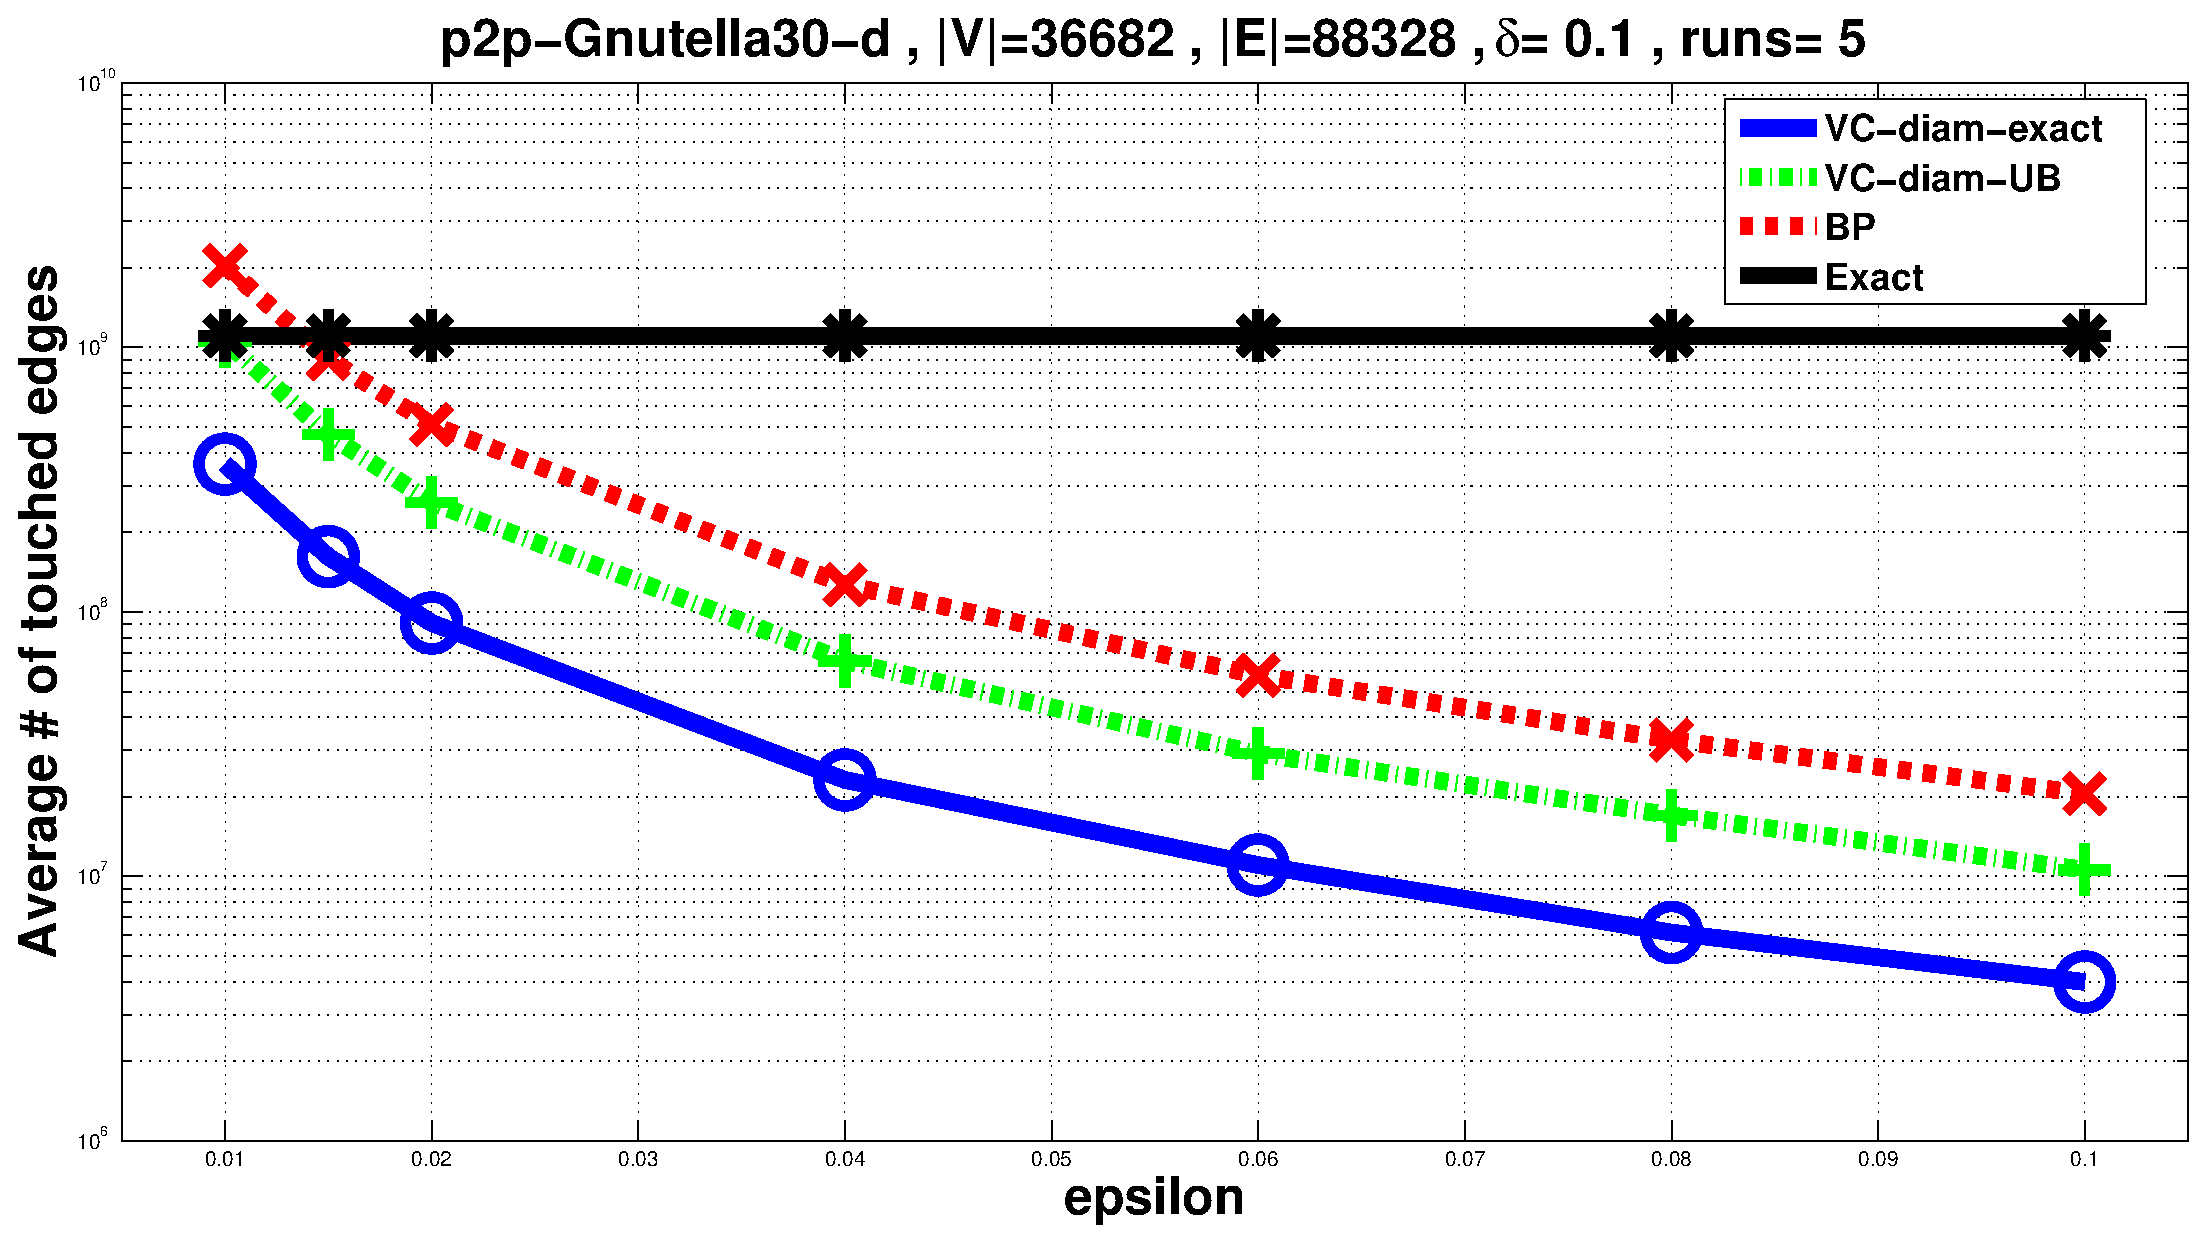
\includegraphics[width=.45\textwidth,keepaspectratio]{p2p-Gnutella30-edges}}
%  \hfil
%  \subfloat[email-Enron
%  (undirected)]{\label{fig:email:edges}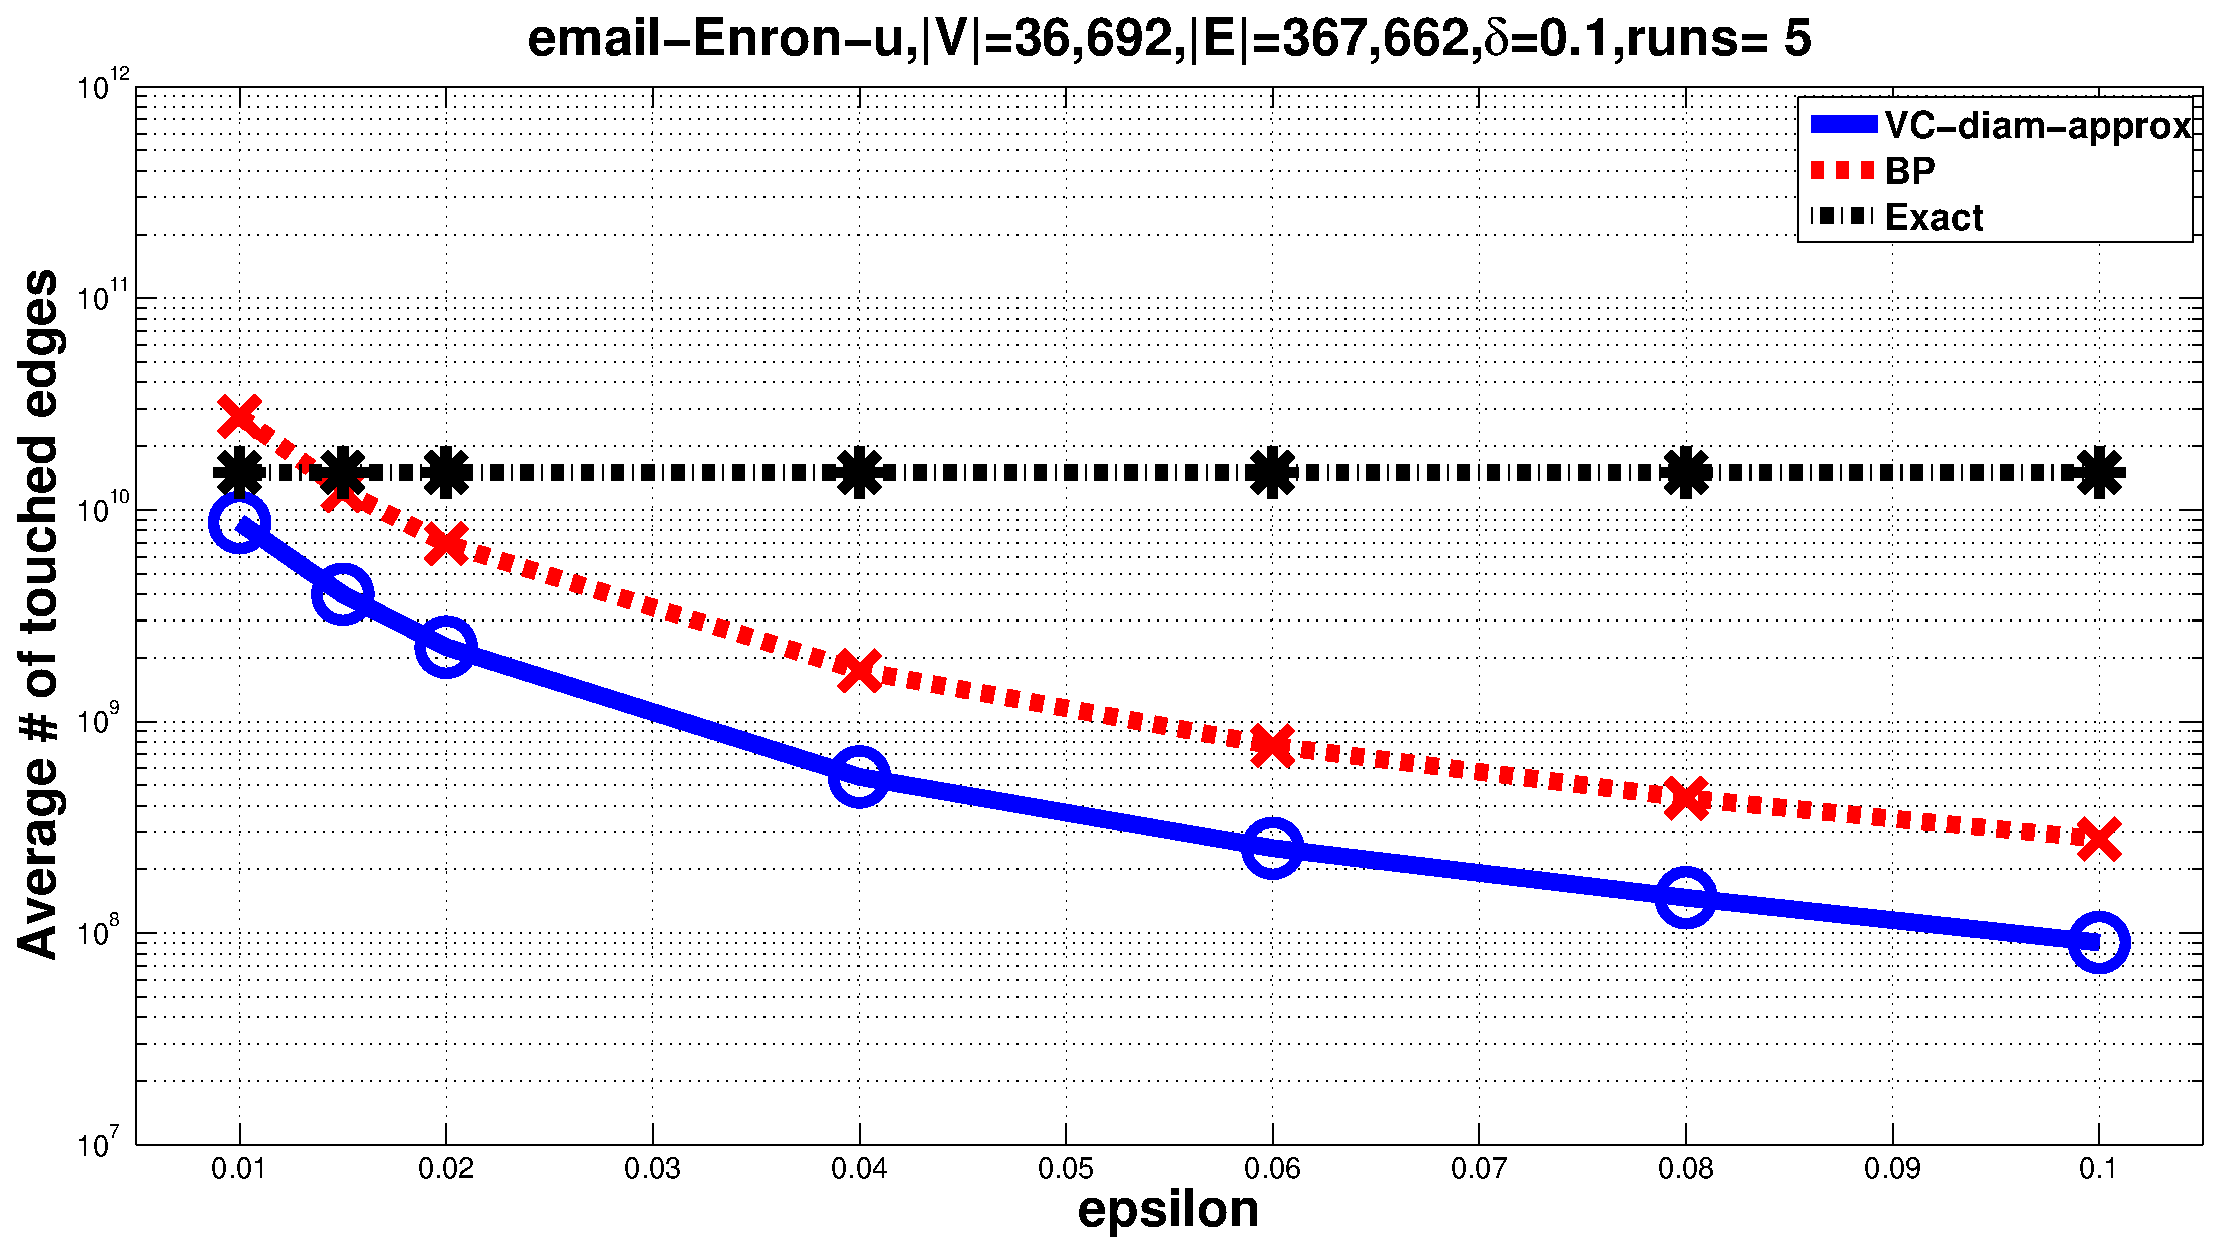
\includegraphics[width=.45\textwidth,keepaspectratio]{email-Enron-edges}}
%  \hfill
%  \label{fig:edges}
%  \caption{Touched edges comparison between $\mathsf{VC}$, $\mathsf{BP}$, and
%  the exact algorithm.}
%\begin{minipage}[b]{0.5\linewidth}
%\flushleft
%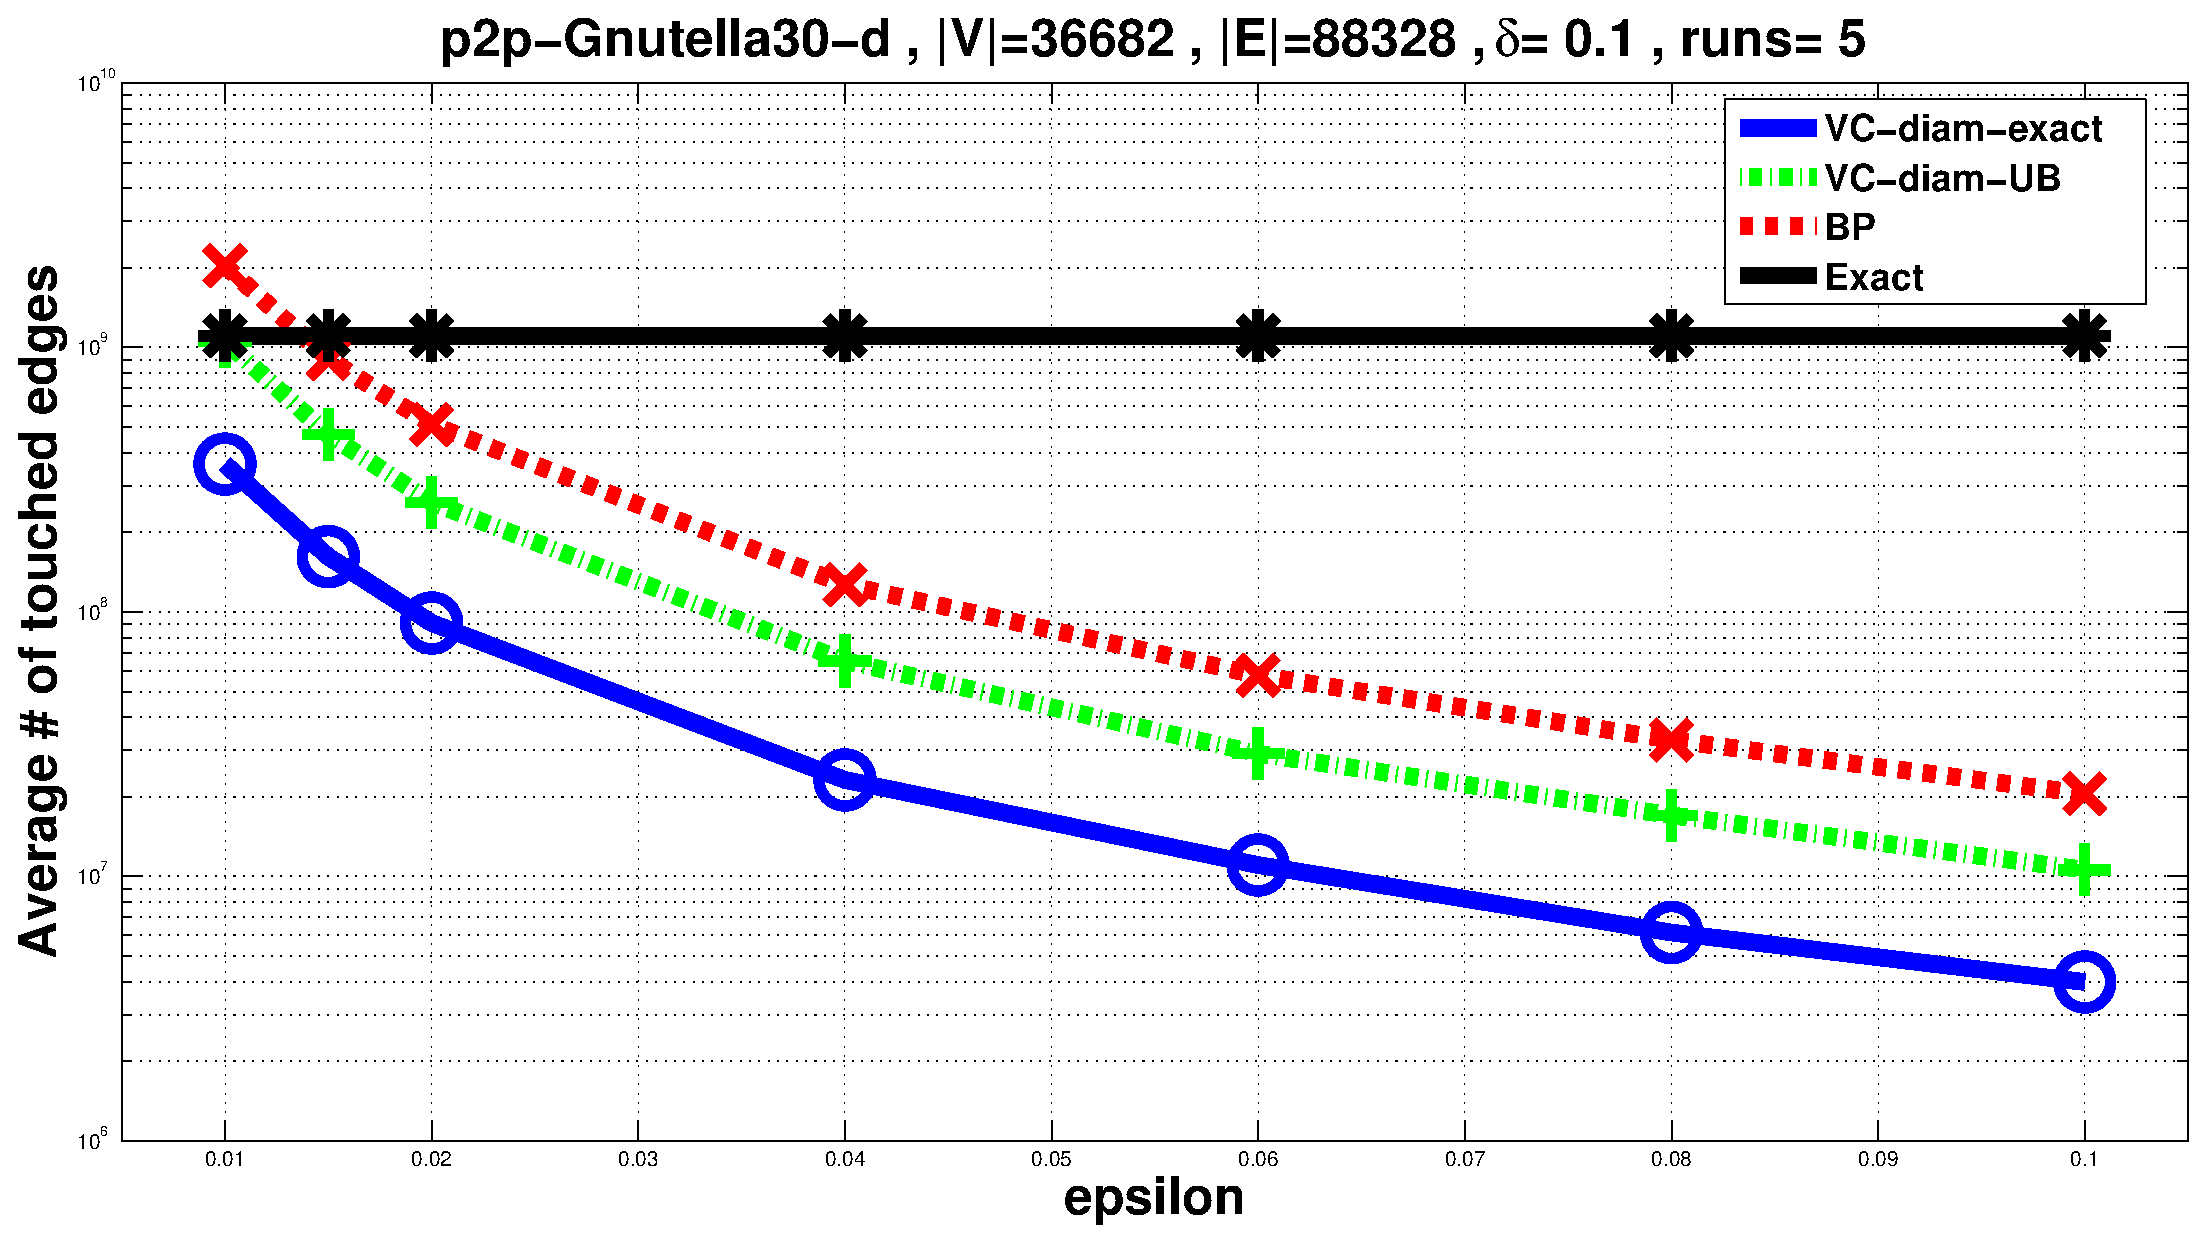
\includegraphics[width=3.8in, keepaspectratio]{p2p-Gnutella30-edges.eps}
%\caption{Touched edges comparison on p2p-Gnutella30} \label{fig:gnutella:edges}
%\end{minipage}%
%\begin{minipage}[b]{0.5\linewidth}
%\centering
%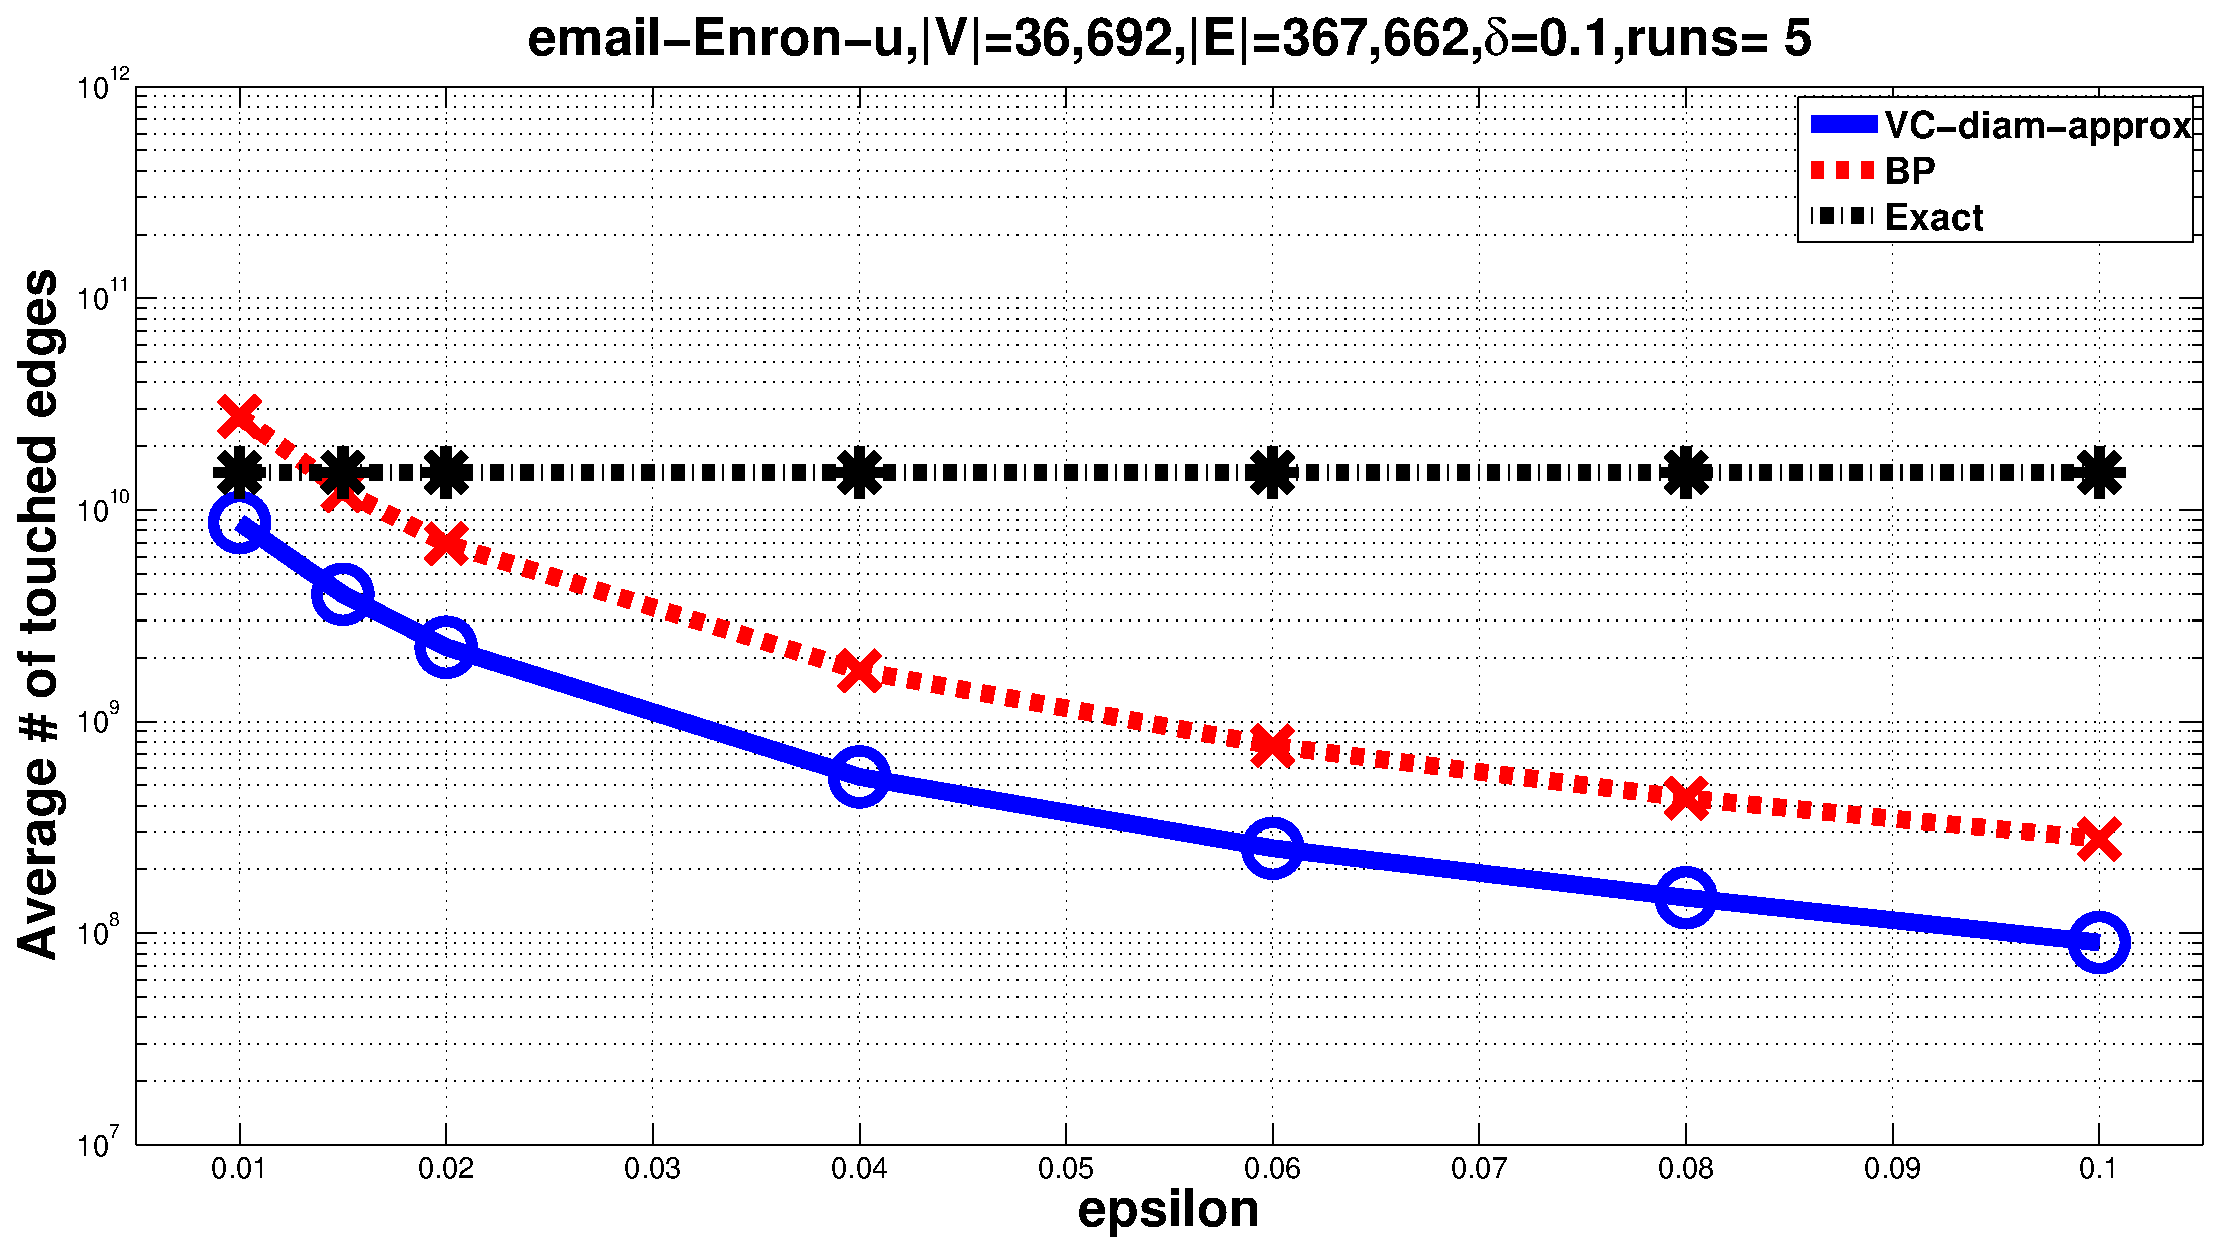
\includegraphics[width=3.8in, keepaspectratio]{email-Enron-edges.eps}
%\caption{Touched edges comparison on email-Enron}\label{fig:email:edges}
%\end{minipage}
%\end{figure*}

\subsection{Scalability}\label{sec:scalability}

In Sect.~\ref{sec:discussion} we argued about the reasons why
Algorithm~\ref{alg:algorithm} is more scalable than $\mathsf{BP}$, while still
offering the same approximation guarantees. To evaluate our argument in practice, we
created a number of graphs of increasing size (1,000 to 100,000 vertices) using
the Barab\'asi-Albert~\citep{BarabasiA99} and run the algorithms on them,
measuring their running time. We report the results in Fig.~\ref{fig:random:time}.
The most-scalable algorithm would be completely independent from the size
(number of vertices) of the graph, corresponding to a flat (horizontal) line in
the plot. Therefore, the less steep the line, the more independent from the
network size would be the corresponding algorithm. From the figure, we can
appreciate that this is the case for $\mathsf{VC}$, which is much more scalable
and independent from the size of the sample than $\mathsf{BP}$. This is very
important, as today's networks are not only huge, but they also grow rapidly,
and algorithms to mine them must scale well with graph size.
\begin{figure}[ht]
  \centering
  \includegraphics[width=.45\textwidth,keepaspectratio]{figures/eps/random-time}
  \caption{Scalability on random~\citet{BarabasiA99} graphs.}
  \label{fig:random:time}
\end{figure}

%\begin{figure*}
%  \centering
%  \hfill
%  \subfloat[Time]{\label{fig:random:time}\includegraphics[width=.45\textwidth,keepaspectratio]{random-time}}
%  \hfill
%  \subfloat[Edges]{\label{fig:random:edges}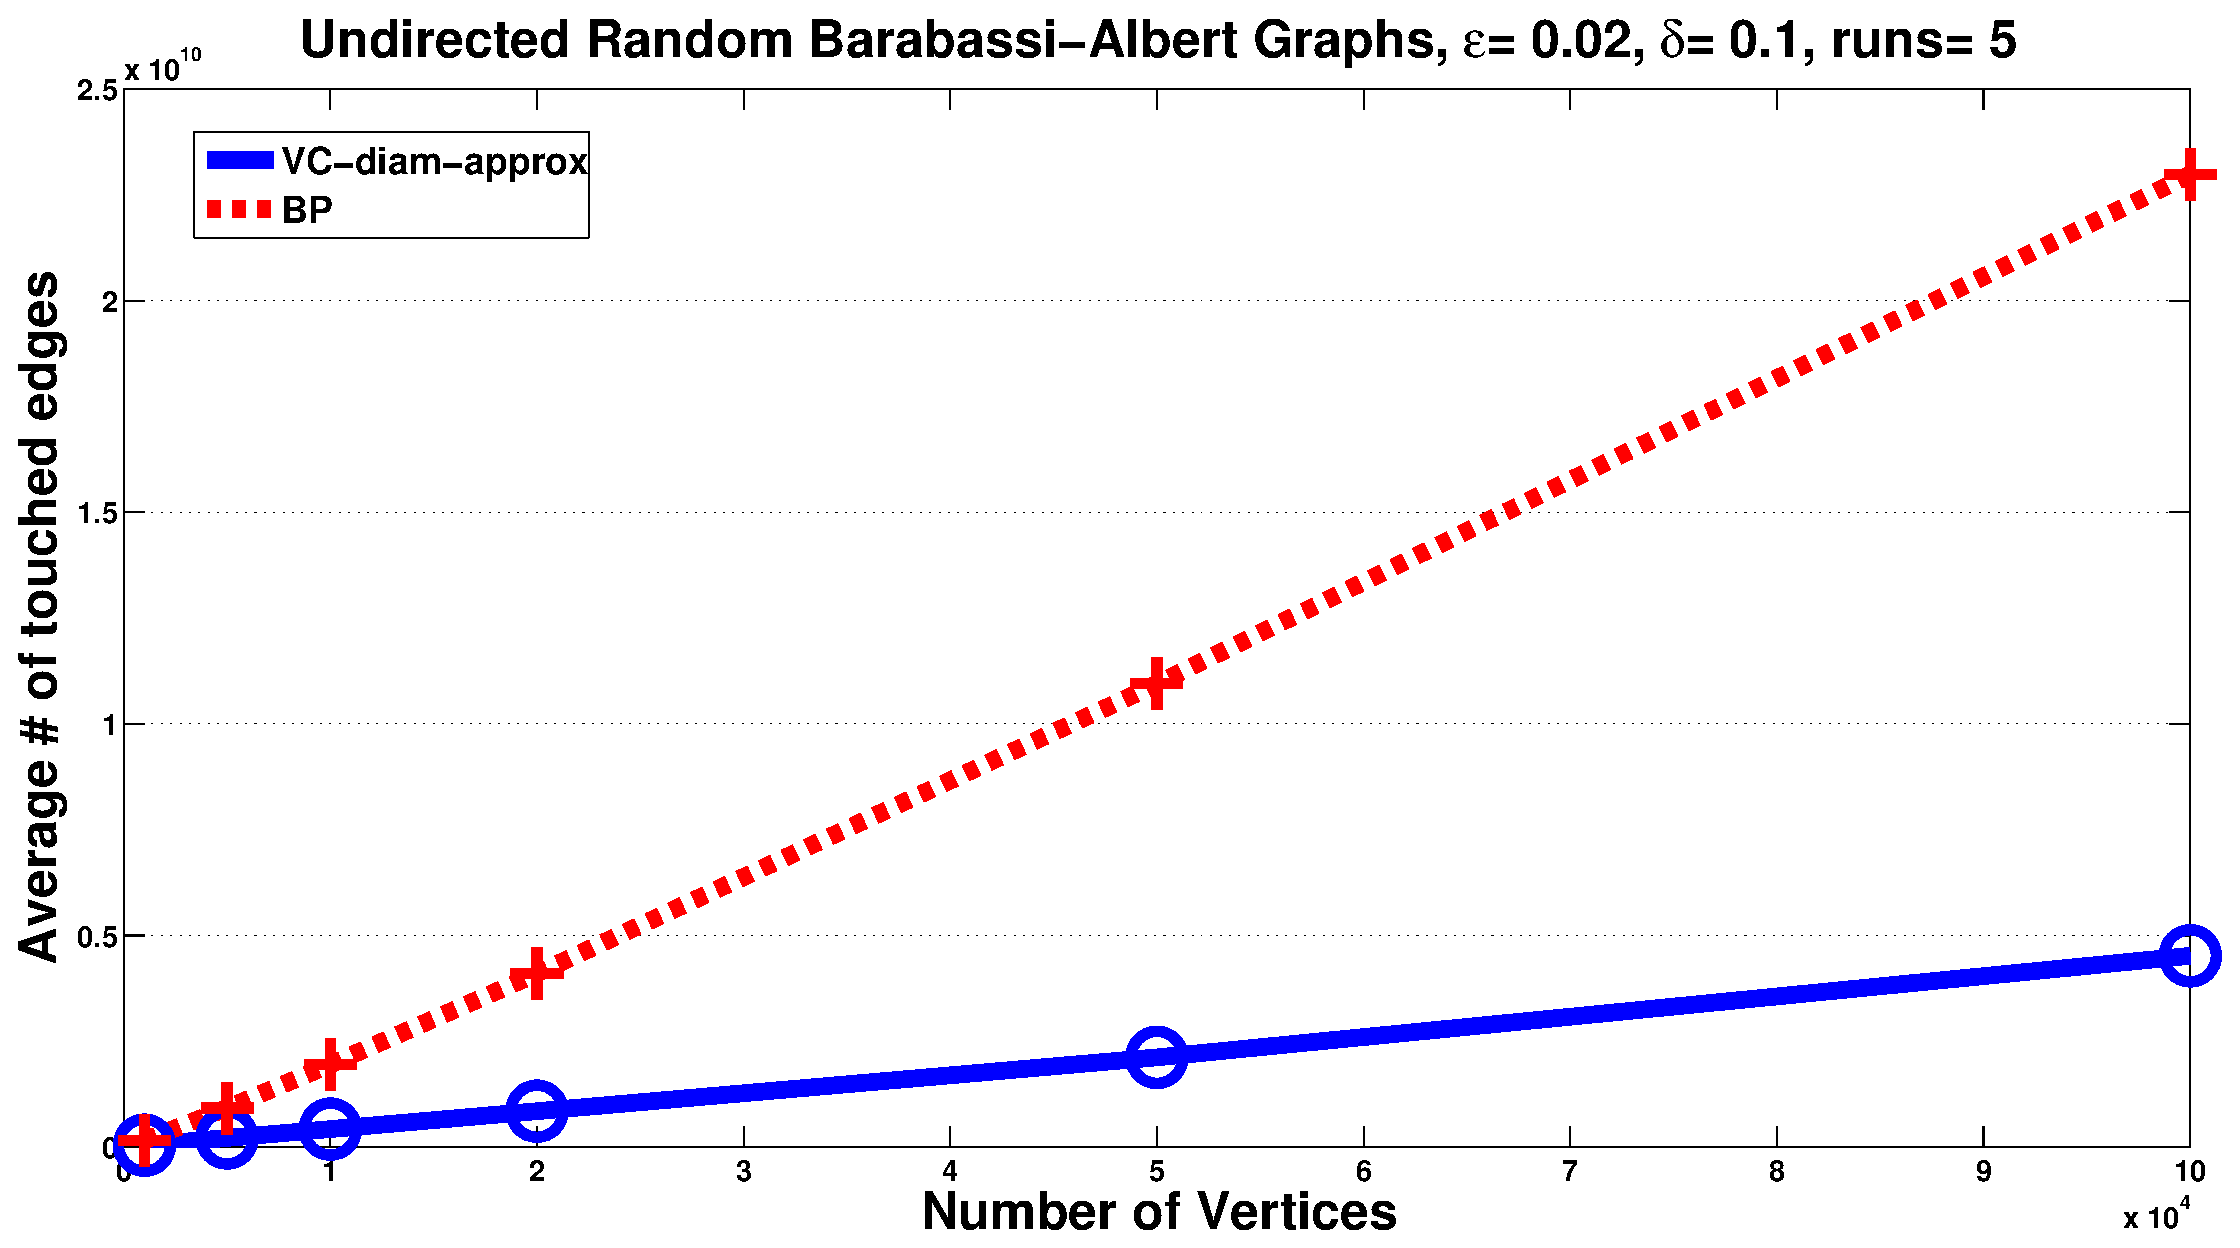
\includegraphics[width=.45\textwidth,keepaspectratio]{random-edges}}
%  \hfill
%  \label{fig:random}
%  \caption{Scalability comparison on random~\citep{BarabasiA99} graphs}
%\end{figure*}
%\begin{minipage}[b]{0.5\linewidth}
%\flushleft
%\includegraphics[width=3.8in, keepaspectratio]{random-time.eps}
%\caption{Scalability on random~\citep{BarabasiA99} graphs (time)}
%\label{fig:random:time}
%\end{minipage}%
%\begin{minipage}[b]{0.5\linewidth}
%\centering
%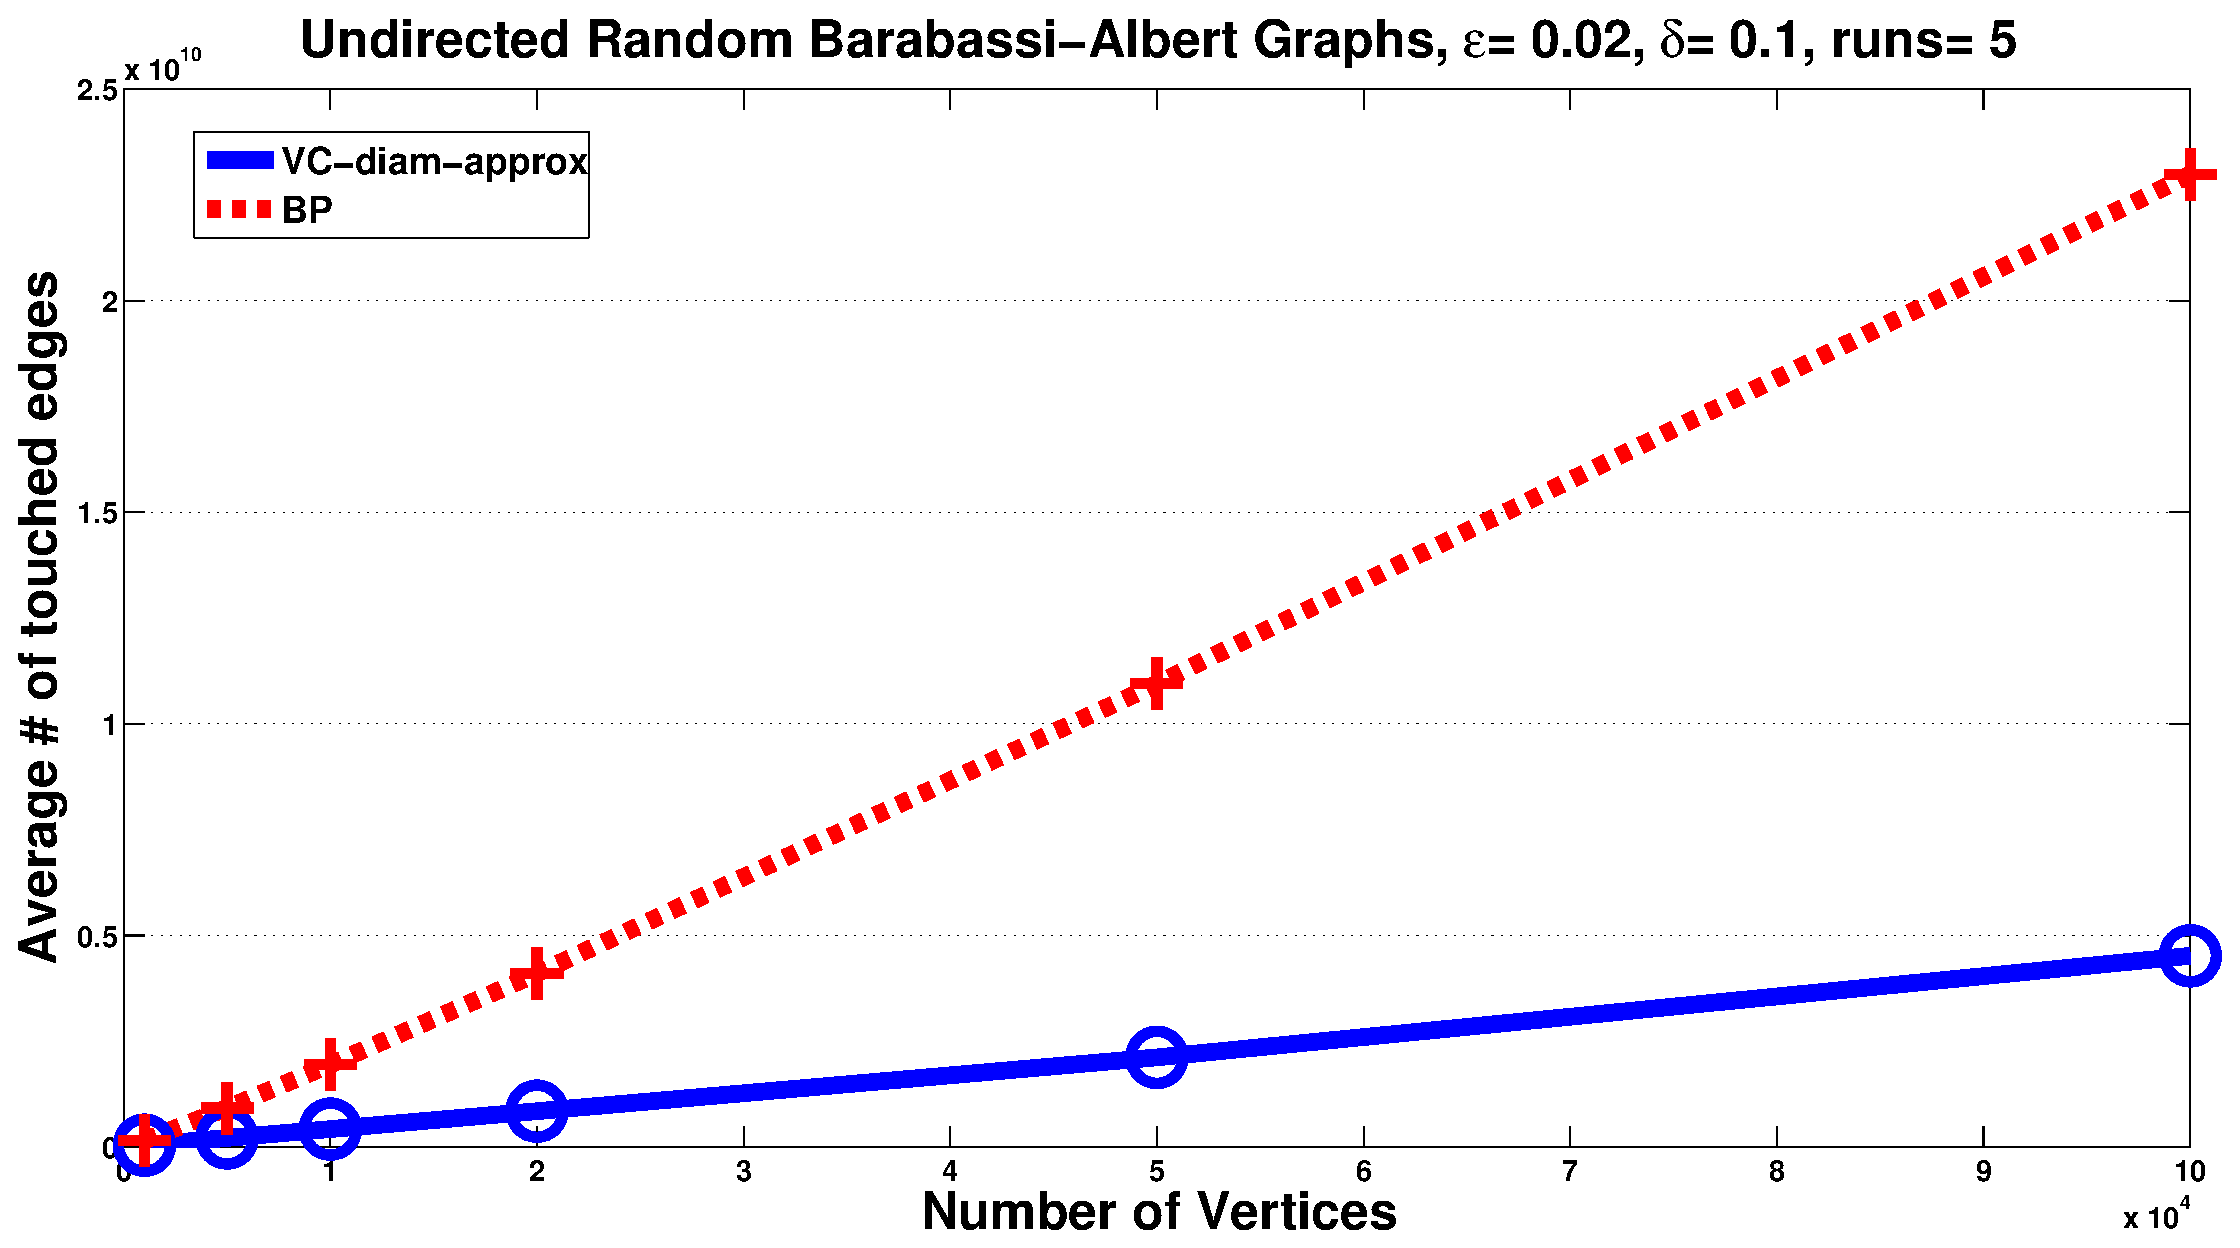
\includegraphics[width=3.8in, keepaspectratio]{random-edges.eps}
%\caption{Scalability on random~\citep{BarabasiA99} graphs (touched edges)}
%\label{fig:random:edges}
%\end{minipage}
%\end{figure*}

\section{Conclusions}\label{sec:concl}
In this work we presented two random-sampling-based algorithms for accurately and
efficiently estimate the betweenness centrality of the (top-$K$) vertices in a
graph, with high probability.
%For very large graphs, exact computation of the
%betweenness centrality is impossible, so one has to resort to an approximation.
Our algorithms are based on a novel application of VC-dimension theory, and
therefore take a different approach than previous ones achieving the same
guarantees~\citep{BrandesP07,GeisbergerSS08,JacobKLPT05}. The number of samples
needed to approximate the betweenness with the desired accuracy and confidence
does not depend on the number of vertices in the graph, but rather on a
characteristic quantity of the network that we call
\emph{vertex-diameter}. In some cases, the sample size is completely
independent from any property of the graph. %, which is interesting and unexpected. %
\ifproof
Our methods can be applied to many variants of betweenness, including edge
betweenness. %
\fi
Our algorithms perform much less work than previously presented methods. %offering
%the same approximation guarantee. 
As a consequence, they are much faster and
scalable, as verified in the extensive experimental
evaluation using many real and artificial graphs. In future work we would like
to explore the possibility of using bidirectional A\textsuperscript{*}
search~\citep{Pohl69,KaindlK97} to further speed up our algorithms.  
%We are also
%interested in extending our methods to generalizations of betweenness
%centrality~\citep{KourtellisASIT12,DolevEP10} and to other centrality measures. 
\vspace{-17pt}
\paragraph*{Acknowledgements} This project was supported, in part, by the
National Science Foundation under award IIS-1247581. We are thankful to Eli
Upfal for his guidance and to the anonymous reviewers whose comments helped us
improving this work.
\vspace{-5pt}

\begin{thebibliography}{35}
\providecommand{\natexlab}[1]{#1}
\providecommand{\url}[1]{\texttt{#1}}
\expandafter\ifx\csname urlstyle\endcsname\relax
  \providecommand{\doi}[1]{doi: #1}\else
  \providecommand{\doi}{doi: \begingroup \urlstyle{rm}\Url}\fi
\vspace{-5pt}
%\providecommand{\natexlab}[1]{#1}
\bibitem[Abraham et~al.(2011)Abraham, Delling, Fiat, Goldberg, and
  Werneck]{AbrahamDFGW11}
%I.~Abraham, D.~Delling, A.~Fiat, A.~V.~Goldberg, and R.~F.~Werneck.
I.~Abraham et al.
\newblock {VC}-dimension and shortest path algorithms.
\newblock ICALP'11, 2011.

\bibitem[Aingworth et~al.(1999)Aingworth, Chekuri, Indyk, and
  Motwani]{AingwordCIM99}
%D.~Aingworth, C.~Chekuri, P.~Indyk, and R.~Motwani.
D.~Aingworth et al.
\newblock Fast estimation of diameter and shortest paths (without matrix
  multiplication).
\newblock \emph{SIAM J.~on Comput.}, 28\penalty0 (4):\penalty0 1167--1181, 1999.

\bibitem[Anthonisse(1971)]{Anthonisse71}
J.~M. Anthonisse.
\newblock The rush in a directed graph.
\newblock TR BN 9/71, Stichting Mathematisch Centrum, Amsterdam,
  Netherlands, 1971.

\bibitem[Bader et~al.(2007)Bader, Kintali, Madduri, and Mihail]{BaderKMM07}
%D.~A.~Bader, S.~Kintali, K.~Madduri, and M.~Mihail.
D.~A.~Bader et al.
\newblock Approximating betweenness centrality.
\newblock WAW'07, 2007.

\bibitem[Barab{\'a}si and Albert(1999)]{BarabasiA99}
A.-L. Barab{\'a}si and R.~Albert.
\newblock Emergence of scaling in random networks.
\newblock \emph{Science}, 286\penalty0 (5439):\penalty0 509--512, 1999.

\bibitem[Boitmanis et~al.(2006)Boitmanis, Freivalds, Ledins, and
  Opmanis]{BoitmanisFL06}
%K.~Boitmanis, K.~Freivalds, P.~Ledins, and R.~Opmanis.
K.~Boitmanis et al.
\newblock Fast and simple approximation of the diameter and radius of a graph.
\newblock WEA'06, 2006.

\bibitem[Borgatti and Everett(2006)]{BorgattiE06}
S.~P.~Borgatti and M.~G.~Everett.
\newblock A graph-theoretic perspective on centrality.
\newblock \emph{Soc.~Net.}, 28\penalty0 (4):\penalty0 466--484, 2006.

\bibitem[Brandes(2001)]{Brandes01}
U.~Brandes.
\newblock A faster algorithm for betweenness centrality.
\newblock \emph{J. Math.~Sociol.}, 25\penalty0 (2):\penalty0 163--177, 2001.

\bibitem[Brandes(2008)]{Brandes08}
U.~Brandes.
\newblock On variants of shortest-path betweenness centrality and their generic
  computation.
\newblock \emph{Soc.~Net.}, 30\penalty0 (2):\penalty0 136--145, 2008.

\bibitem[Brandes and Pich(2007)]{BrandesP07}
U.~Brandes and C.~Pich.
\newblock Centrality estimation in large networks.
\newblock \emph{Intl.~J. Bifurc.~and Chaos}, 17\penalty0 (07):\penalty0
2303--2318, 2007.

\bibitem[Cs\'{a}rdi and Nepusz(2006)]{igraph}
G.~Cs\'{a}rdi and T.~Nepusz.
\newblock The igraph software package for complex network research.
\newblock \emph{InterJournal}, Complex Sys.:\penalty0 1695, 2006.
\newblock URL \url{http://igraph.sf.net}.

\bibitem[Dolev et~al.(2010)Dolev, Elovici, and Puzis]{DolevEP10}
%S.~Dolev, Y.~Elovici, and R.~Puzis.
S.~Dolev et al.
\newblock Routing betweenness centrality.
\newblock \emph{J. ACM}, 57\penalty0 (4):\penalty0 25:1--25:27, May 2010.

\bibitem[Eppstein and Wang(2004)]{EppsteinW04}
D.~Eppstein and J.~Wang.
\newblock Fast approximation of centrality.
\newblock \emph{J.~Graph Alg.~and Appl.}, 8\penalty0
  (1):\penalty0 39--45, 2004.

\bibitem[Freeman(1977)]{Freeman77}
L.~C. Freeman.
\newblock A set of measures of centrality based on betweenness.
\newblock \emph{Sociometry}, 40:\penalty0 35--41, 1977.

\bibitem[Geisberger et~al.(2008)Geisberger, Sanders, and
  Schultes]{GeisbergerSS08}
%R.~Geisberger, P.~Sanders, and D.~Schultes.
R.~Geisberger et al.
\newblock Better approximation of betweenness centrality.
\newblock ALENEX'08, 2008.

\bibitem[Har-Peled and Sharir(2011)]{HarPS11}
S.~Har-Peled and M.~Sharir.
\newblock Relative $(p,\varepsilon)$-approximations in geometry.
\newblock \emph{Discr.~\& Comput.~Geom.}, 45\penalty0 (3):\penalty0
  462--496, 2011.

\bibitem[Hoeffding(1963)]{Hoeffding63}
W.~Hoeffding.
\newblock Probability inequalities for sums of bounded random variables.
\newblock \emph{J.~Am.~Stat.~Assoc.}, 58\penalty0
  (301):\penalty0 13--30, 1963.

\bibitem[Jacob et~al.(2005)Jacob, Kosch{\"u}tzki, Lehmann, Peeters, and
  Tenfelde-Podehl]{JacobKLPT05}
%R.~Jacob, D.~Kosch{\"u}tzki, K.~Lehmann, L.~Peeters, and D.~Tenfelde-Podehl.
R.~Jacob et al.
\newblock Algorithms for centrality indices.
\newblock \emph{LNCS}, 3418:\penalty0 62--82, 2005.

\bibitem[Kaindl and Kainz(1997)]{KaindlK97}
H.~Kaindl and G.~Kainz.
\newblock Bidirectional heuristic search reconsidered.
\newblock \emph{J. Artif. Intell. Res.}, 7:\penalty0 283--317, 1997.

\bibitem[Kourtellis et~al.(2012)Kourtellis, Alahakoon, Simha, Iamnitchi, and
  Tripathi]{KourtellisASIT12}
%N.~Kourtellis, T.~Alahakoon, R.~Simha, A.~Iamnitchi, and R.~Tripathi.
Kourtellis et al.
\newblock Identifying high betweenness centrality nodes in large social
  networks.
\newblock \emph{Soc.~Net.~Analysis and Mining}, pages 1--16, 2012.

\bibitem[Kranakis et~al.(1997)Kranakis, Krizanc, Ruf, Urrutia, and
  Woeginger]{KranakisKRUW97}
%E.~Kranakis, D.~Krizanc, B.~Ruf, J.~Urrutia, and G.~Woeginger.
Kranakis et al.
\newblock The {VC}-dimension of set systems defined by graphs.
\newblock \emph{Discr. Appl. Math.}, 77\penalty0 (3):\penalty0
  237--257, 1997.

\bibitem[Li et~al.(2001)Li, Long, and Srinivasan]{LiLS01}
%Y.~Li, P.~M. Long, and A.~Srinivasan.
Y.~Li et al.
\newblock Improved bounds on the sample complexity of learning.
\newblock \emph{J.~Comp.~and~Sys.~Sci.}, 62\penalty0
  (3):\penalty0 516--527, 2001.

\bibitem[Lim et~al.(2011)Lim, Menasche, Ribeiro, Towsley, and Basu]{LimMRTB11}
%Y.-s. Lim, D.~Menasche, B.~Ribeiro, D.~Towsley, and P.~Basu.
Y.-s. Lim et al.
\newblock Online estimating the k central nodes of a network.
\newblock NSW'11, 2011

\bibitem[L\"{o}ffler and Phillips(2009)]{LofflerP09}
M.~L\"{o}ffler and J.~M. Phillips.
\newblock Shape fitting on point sets with probability distributions.
\newblock ESA'09, 2009.

\bibitem[Maiya and Berger-Wolf(2010)]{MaiyaBW10}
A.~Maiya and T.~Berger-Wolf.
\newblock Online sampling of high centrality individuals in social networks.
\newblock PAKDD'10, 2010.

\bibitem[Mitzenmacher and Upfal(2005)]{MitzenmacherU05}
M.~Mitzenmacher and E.~Upfal.
\newblock \emph{Probability and Computing: Randomized Algorithms and
  Probabilistic Analysis}.
\newblock Cambridge University Press, 2005.

\bibitem[Mohri et~al.(2012)Mohri, Rostamizadeh, and Talwalkar]{MohriRT12}
%M.~Mohri, A.~Rostamizadeh, and A.~Talwalkar.
M.~Mohri et al.
\newblock \emph{Foundations of Machine Learning}.
\newblock The MIT Press, 2012.

\bibitem[Newman(2010)]{Newman10}
M.~E.~J.~Newman.
\newblock \emph{Networks - An Introduction}.
\newblock Oxford University Press, 2010.

\bibitem[Pfeffer and Carley(2012)]{PfefferC12}
J.~Pfeffer and K.~M.~Carley.
\newblock k-centralities: local approximations of global measures based on
  shortest paths.
\newblock WWW'12, 2012.

\bibitem[Pohl(1969)]{Pohl69}
I.~Pohl.
\newblock \emph{Bidirectional Heuristic Search in Path Problems}.
\newblock PhD thesis, Stanford University, 1969.

\bibitem[Riondato and Kornaropoulos(2013)]{RiondatoK13}
 M.~Riondato and E.~M.~Kornaropoulos
 \newblock Fast Approximation of Betweenness Centrality through Sampling.
 \newblock (extended version) \url{http://cs.brown.edu/~matteo/papers/RiondatoKornarop-BetweennessSampling.pdf}, 2013.

\bibitem[Roditty and Williams(2012)]{RodittyW12}
L.~Roditty and V.~V.~Williams.
\newblock Approximating the diameter of a graph.
\newblock \emph{CoRR abs/1207.3622}, 2012.

\bibitem[Sariy\"{u}ce et~al.(2013 (to appear))Sariy\"{u}ce, Saule, Kaya, and
  Catalyurek]{SaryuceSKC13}
%A.~E.~Sariy\"{u}ce, E.~Saule, K.~Kaya, and U.~V.~Catalyurek.
A.~E.~Sariy\"{u}ce et al.
\newblock Shattering and compressing networks for betweenness centrality.
\newblock SDM'13, 2013.

\bibitem[Vapnik and Chervonenkis(1971)]{VapnikC71}
V.~N.~Vapnik and A.~J.~Chervonenkis.
\newblock On the uniform convergence of relative frequencies of events to their
  probabilities.
\newblock \emph{Theory~of Prob.~and its Appl.}, 16\penalty0
  (2):\penalty0 264--280, 1971.

\end{thebibliography}
%\fi

%\bibliographystyle{abbrvnat}
%\bibliography{bidirectionalsearch,centrality,diamapprox,various,vcmine,vcgraph}

\end{document}

